\PassOptionsToPackage{unicode=true}{hyperref} % options for packages loaded elsewhere
\PassOptionsToPackage{hyphens}{url}
\PassOptionsToPackage{dvipsnames,svgnames*,x11names*}{xcolor}
%
\documentclass[11pt,]{report}
\usepackage{lmodern}
\usepackage{setspace}
\setstretch{1.5}
\usepackage{amssymb,amsmath}
\usepackage{ifxetex,ifluatex}
\usepackage{fixltx2e} % provides \textsubscript
\ifnum 0\ifxetex 1\fi\ifluatex 1\fi=0 % if pdftex
  \usepackage[T1]{fontenc}
  \usepackage[utf8]{inputenc}
  \usepackage{textcomp} % provides euro and other symbols
\else % if luatex or xelatex
  \usepackage{unicode-math}
  \defaultfontfeatures{Ligatures=TeX,Scale=MatchLowercase}
\fi
% use upquote if available, for straight quotes in verbatim environments
\IfFileExists{upquote.sty}{\usepackage{upquote}}{}
% use microtype if available
\IfFileExists{microtype.sty}{%
\usepackage[]{microtype}
\UseMicrotypeSet[protrusion]{basicmath} % disable protrusion for tt fonts
}{}
\IfFileExists{parskip.sty}{%
\usepackage{parskip}
}{% else
\setlength{\parindent}{0pt}
\setlength{\parskip}{6pt plus 2pt minus 1pt}
}
\usepackage{xcolor}
\usepackage{hyperref}
\hypersetup{
            pdftitle={Shrinking Characteristics of Precision Matrix Estimators: An Illustration via Regression},
            pdfauthor={Matt Galloway},
            colorlinks=true,
            linkcolor=Maroon,
            citecolor=Blue,
            urlcolor=Blue,
            breaklinks=true}
\urlstyle{same}  % don't use monospace font for urls
\usepackage[left = 1in, right = 1in, top = 1in, bottom = 1in]{geometry}
\usepackage{color}
\usepackage{fancyvrb}
\newcommand{\VerbBar}{|}
\newcommand{\VERB}{\Verb[commandchars=\\\{\}]}
\DefineVerbatimEnvironment{Highlighting}{Verbatim}{commandchars=\\\{\}}
% Add ',fontsize=\small' for more characters per line
\usepackage{framed}
\definecolor{shadecolor}{RGB}{248,248,248}
\newenvironment{Shaded}{\begin{snugshade}}{\end{snugshade}}
\newcommand{\AlertTok}[1]{\textcolor[rgb]{0.94,0.16,0.16}{#1}}
\newcommand{\AnnotationTok}[1]{\textcolor[rgb]{0.56,0.35,0.01}{\textbf{\textit{#1}}}}
\newcommand{\AttributeTok}[1]{\textcolor[rgb]{0.77,0.63,0.00}{#1}}
\newcommand{\BaseNTok}[1]{\textcolor[rgb]{0.00,0.00,0.81}{#1}}
\newcommand{\BuiltInTok}[1]{#1}
\newcommand{\CharTok}[1]{\textcolor[rgb]{0.31,0.60,0.02}{#1}}
\newcommand{\CommentTok}[1]{\textcolor[rgb]{0.56,0.35,0.01}{\textit{#1}}}
\newcommand{\CommentVarTok}[1]{\textcolor[rgb]{0.56,0.35,0.01}{\textbf{\textit{#1}}}}
\newcommand{\ConstantTok}[1]{\textcolor[rgb]{0.00,0.00,0.00}{#1}}
\newcommand{\ControlFlowTok}[1]{\textcolor[rgb]{0.13,0.29,0.53}{\textbf{#1}}}
\newcommand{\DataTypeTok}[1]{\textcolor[rgb]{0.13,0.29,0.53}{#1}}
\newcommand{\DecValTok}[1]{\textcolor[rgb]{0.00,0.00,0.81}{#1}}
\newcommand{\DocumentationTok}[1]{\textcolor[rgb]{0.56,0.35,0.01}{\textbf{\textit{#1}}}}
\newcommand{\ErrorTok}[1]{\textcolor[rgb]{0.64,0.00,0.00}{\textbf{#1}}}
\newcommand{\ExtensionTok}[1]{#1}
\newcommand{\FloatTok}[1]{\textcolor[rgb]{0.00,0.00,0.81}{#1}}
\newcommand{\FunctionTok}[1]{\textcolor[rgb]{0.00,0.00,0.00}{#1}}
\newcommand{\ImportTok}[1]{#1}
\newcommand{\InformationTok}[1]{\textcolor[rgb]{0.56,0.35,0.01}{\textbf{\textit{#1}}}}
\newcommand{\KeywordTok}[1]{\textcolor[rgb]{0.13,0.29,0.53}{\textbf{#1}}}
\newcommand{\NormalTok}[1]{#1}
\newcommand{\OperatorTok}[1]{\textcolor[rgb]{0.81,0.36,0.00}{\textbf{#1}}}
\newcommand{\OtherTok}[1]{\textcolor[rgb]{0.56,0.35,0.01}{#1}}
\newcommand{\PreprocessorTok}[1]{\textcolor[rgb]{0.56,0.35,0.01}{\textit{#1}}}
\newcommand{\RegionMarkerTok}[1]{#1}
\newcommand{\SpecialCharTok}[1]{\textcolor[rgb]{0.00,0.00,0.00}{#1}}
\newcommand{\SpecialStringTok}[1]{\textcolor[rgb]{0.31,0.60,0.02}{#1}}
\newcommand{\StringTok}[1]{\textcolor[rgb]{0.31,0.60,0.02}{#1}}
\newcommand{\VariableTok}[1]{\textcolor[rgb]{0.00,0.00,0.00}{#1}}
\newcommand{\VerbatimStringTok}[1]{\textcolor[rgb]{0.31,0.60,0.02}{#1}}
\newcommand{\WarningTok}[1]{\textcolor[rgb]{0.56,0.35,0.01}{\textbf{\textit{#1}}}}
\usepackage{longtable,booktabs}
% Fix footnotes in tables (requires footnote package)
\IfFileExists{footnote.sty}{\usepackage{footnote}\makesavenoteenv{longtable}}{}
\setlength{\emergencystretch}{3em}  % prevent overfull lines
\providecommand{\tightlist}{%
  \setlength{\itemsep}{0pt}\setlength{\parskip}{0pt}}
\setcounter{secnumdepth}{5}
% Redefines (sub)paragraphs to behave more like sections
\ifx\paragraph\undefined\else
\let\oldparagraph\paragraph
\renewcommand{\paragraph}[1]{\oldparagraph{#1}\mbox{}}
\fi
\ifx\subparagraph\undefined\else
\let\oldsubparagraph\subparagraph
\renewcommand{\subparagraph}[1]{\oldsubparagraph{#1}\mbox{}}
\fi

% set default figure placement to htbp
\makeatletter
\def\fps@figure{htbp}
\makeatother

\usepackage{booktabs}
\usepackage{amsthm}
\usepackage{amsmath}
\usepackage{fancyhdr} % Required for custom headers
\usepackage{lastpage} % Required to determine the last page for the footer
\usepackage{extramarks} % Required for headers and footers
\usepackage{graphicx} % Required for knitr::include_graphics
\makeatletter
\def\thm@space@setup{%
  \thm@preskip=8pt plus 2pt minus 4pt
  \thm@postskip=\thm@preskip
}
\makeatother
\pagestyle{fancy}
% \pagestyle{empty}
% \usepackage[left]{lineno} % line number package
% \linenumbers % line number command
\usepackage[]{natbib}
\bibliographystyle{apalike}

\title{Shrinking Characteristics of Precision Matrix Estimators: An Illustration via Regression}
\author{Matt Galloway}
\date{2019-05-01}

\usepackage{amsthm}
\newtheorem{theorem}{Theorem}[chapter]
\newtheorem{lemma}{Lemma}[chapter]
\newtheorem{corollary}{Corollary}[chapter]
\newtheorem{proposition}{Proposition}[chapter]
\newtheorem{conjecture}{Conjecture}[chapter]
\theoremstyle{definition}
\newtheorem{definition}{Definition}[chapter]
\theoremstyle{definition}
\newtheorem{example}{Example}[chapter]
\theoremstyle{definition}
\newtheorem{exercise}{Exercise}[chapter]
\theoremstyle{remark}
\newtheorem*{remark}{Remark}
\newtheorem*{solution}{Solution}
\let\BeginKnitrBlock\begin \let\EndKnitrBlock\end
\begin{document}
\maketitle

{
\hypersetup{linkcolor=}
\setcounter{tocdepth}{1}
\tableofcontents
}
\hypertarget{preface}{%
\chapter*{Preface}\label{preface}}


I would like to thank my advisor Professor Adam Rothman for his guidance and support this past year. His enthusiasm towards this research area is ultimately what got me interested and I truly enjoyed having the opportunity to learn from him.

My parents also deserve a note of appreciation and thanks -- one probably much longer than this. Graduate school would not have been possible without their love and encouragement.

\hypertarget{intro}{%
\chapter{Introduction}\label{intro}}

Inferential statistics consists of two primary components: estimation and prediction. Estimation refers to the process by which we infer values, properties and behavior about individual parameters in our model. Prediction, on the other hand, refers to the process by which we draw inference about an event that has not-yet occurred. The latter component is abundant in industry where the demand to predict stock prices, movies individuals prefer, and even to predict new friend connections in a network has sparked huge investments in research and given rise to research groups whose primary goal is pushing the bounds and developing new predictive models.

However, though most attention is directed towards prediction, these two components are not distinct. In fact, the success and reliability of many predictive models is contingent upon good, efficient parameter estimation. Many of these models require the estimation of a precision matrix - the inverse of the covariance matrix (frequently denoted as \(\Omega\)) - that establishes the interaction and covariance between random variables. For this reason, the last decade has seen an ever-expanding community devoted to precision matrix estimation.

Among this community of researchers is Professor Adam Rothman and Aaron Molstad, Ph.D.~whose research will be a focal point of this manuscript. The two have published work on indirect multivariate linear regression (\citet{molstad2016indirect}) and classification with matrix-valued predictors (\citet{molstad2018penalized}) but the focus of this manuscript is their 2017 paper titled \emph{Shrinking Characteristics of Precision Matrix Estimators} (\citet{molstad2017shrinking}). In it, they outline a framework to shrink a \emph{characteristic} of a precision matrix - a concept that exploits the fact that in many predictive models estimation of the precision matrix is only necessary through its product with another feature. They write in their manuscript that ``to fit many predictive models, only a characteristic of the population precision matrix needs to be estimated\ldots{} In binary linear discriminant analysis, the population precision matrix is needed for prediction only through the product of the precision matrix and the difference between the two conditional distribution mean vectors.'' The purpose of the research detailed here began with the desire to expand on this concept and to explore avenues that were mentioned but were not further investigated.

One of the research directions mentioned in the original paper was the application of their framework to regression. Utilizing the fact that the population regression coefficient matrix \(\beta \equiv \Omega_{x}\Sigma_{xy}\) (where \(\Sigma_{xy}\) is the cross-covariance matrix between the predictors, \(X\), and the responses, \(Y\), and \(\Omega_{x}\) is the precision matrix for \(X\)), their framework allows for the simultaneous estimation of \(\beta\) and \(\Omega_{x}\) with an embedded assumption potentially useful for superior prediction performance. In close communication and collaboration with Professor Rothman, we wanted to explore this research direction further. However, in order to build upon their work and contribute new material, there were a number of concepts that needed to be learned along the way and this document will follow that journey.

We will begin chapter two with a brief introduction to precision matrix estimation and the gaussian log-likelihood function. This section will mention popular estimation methods and algorithms but most discussion will be directed towards the ADMM algorithm. Discussion of the ADMM algorithm will be useful as we begin detailing the shrinking characteristics of precision matrix estimators framework (which may be referred to as SCPME), the so-called augmented ADMM algorithm, and later the framework's application to regression. Lastly, the document will end with two brief tutorials for the R packages \texttt{ADMMsigma} and \texttt{SCPME}. These packages were developed by myself to aid in simulation experiments and make it easier to branch into related research directions. Both packages have since been published on CRAN.

\hypertarget{notation-and-definitions}{%
\subsection{Notation and Definitions}\label{notation-and-definitions}}

For strictly positive integers \(n\) and \(p\), we will denote \(\mathbb{R}^{n \times p}\) as the class of real matrices with dimenson \(n \times p\). The class of real, symmetric matrices with dimension \(p \times p\) will be denoted as \(\mathbb{S}^{p}\) and \(\mathbb{S}^{p}_{+}\) if we further require the object to be positive definite. The sample size and dimension of the predictor vector in a given data set will most often be denoted as \(n\) and \(p\), respectively. If the dimension of the response vector exceeds one, we will denote it as \(r\).

Most matrices will take the form of either \(\Sigma\), the population covariance matrix, or \(\Omega\), the population precision matrix. Note that the precision matrix is simply the inverse of the covariance matrix (\(\Omega \equiv \Sigma^{-1}\)) and a subscript may be added to each if more than two random variables are considered in a problem (\(\Omega_{x}\)). A subscript star may also be added if the object is oracle - or known - a priori (\(\Omega_{*}\)). The oracle's estimator that optimizes a pre-specified objective function will be denoted with a hat (\(\hat{\Omega}\)).

There will be significant matrix algebra notation throughout the manuscript. The trace operator sums the diagonal elements of a matrix and will take the form \(tr\left(\cdot\right)\) and the \emph{exponential} trace operator will be denoted similarly as \(etr\left(\cdot\right)\). The vector operator, \(vec\left(\cdot\right)\), stacks the columns of a matrix into a column vector. The determinant of a matrix \(\mathbf{A}\) will be denoted as \(\left|\mathbf{A}\right|\) but may also take the form \(det\left(\mathbf{A}\right)\). The kronecker product of two matrices \(\mathbf{A}\) and \(\mathbf{B}\) will be denoted as \(\mathbf{A} \otimes \mathbf{B}\) and the element-wise product will be denoted as \(\mathbf{A} \circ \mathbf{B}\). Lastly, the Frobenius norm which sums the square of all entries in a matrix will be denoted as \(\left\|\mathbf{A}\right\|_{F}\) and we will define \(\left\|\mathbf{A}\right\|_{1} := \sum_{i, j}\left|\mathbf{A}_{ij}\right|\) where the \(i\)-\(j\)th element in matrix \(\mathbf{A}\) is typically denoted as \(\left(\mathbf{A}\right)_{ij}\) or simply \(\mathbf{A}_{ij}\).

\hypertarget{precision-matrix-estimation}{%
\chapter{Precision Matrix Estimation}\label{precision-matrix-estimation}}

\hypertarget{background}{%
\section{Background}\label{background}}

The foundation of much of the precision matrix estimation literature is the gaussian negative log-likelihood. Consider the case where we observe \(n\) independent, identically distributed (iid) copies of the random variable \(X\), where the \(i\)th observation \(X_{i} \in \mathbb{R}^{p}\) is normally distributed with mean, \(\mu\), and variance, \(\Omega^{-1}\). That is, \(X_{i}\) follows a \(p\)-dimensional normal distribution which is typically denoted as \(X_{i} \sim N_{p}\left( \mu, \Omega^{-1} \right)\). By definition, this multivariate formulation implies the probability distribution function, \(f\), is of the form

\begin{equation} 
  f\left(X_{i}; \mu, \Omega\right) = (2\pi)^{-p/2}\left| \Omega \right|^{1/2}\exp\left[ -\frac{1}{2}\left( X_{i} - \mu \right)'\Omega\left( X_{i} - \mu \right) \right] 
\label{eq:normallikone}\notag
\end{equation}

Furthermore, because we assume that each observation is independent, the probability distribution function for all \(n\) observations \(X_{1}, ..., X_{n}\) is equal to

\begin{equation} 
\begin{split}
  f\left(X_{1}, ..., X_{n}; \mu, \Omega\right) &= \prod_{i = 1}^{n}(2\pi)^{-p/2}\left| \Omega \right|^{1/2}\exp\left[ -\frac{1}{2}\left( X_{i} - \mu \right)'\Omega\left( X_{i} - \mu \right) \right] \\
  &= (2\pi)^{-np/2}\left| \Omega \right|^{n/2}\mbox{etr}\left[ -\frac{1}{2}\sum_{i = 1}^{n}\left( X_{i} - \mu \right)\left( X_{i} - \mu \right)'\Omega \right]
\end{split}
\label{eq:normallik}\notag
\end{equation}

Therefore, the gaussian log-likelihood, \(l\), for \(\mu\) and \(\Omega\) given \(X = (X_{1}, .., X_{n})\) can be written as

\begin{equation}
  l(\mu, \Omega | X) = constant + \frac{n}{2}\log\left| \Omega \right| - tr\left[ \frac{1}{2}\sum_{i = 1}^{n}\left(X_{i} - \mu \right)\left(X_{i} - \mu \right)'\Omega \right]
\label{eq:normalloglik}\notag
\end{equation}

The estimator for \(\mu\) that maximizes the log-likelihood is \(\hat{\mu}^{mle} = \bar{X} \equiv \sum_{i = 1}^{n}X_{i}/n\), so that the partially maximized gaussian log-likelihood function for \(\Omega\) is

\begin{equation}
\begin{split}
  l(\Omega | X) &= \frac{n}{2}\log\left| \Omega \right| - tr\left[ \frac{1}{2}\sum_{i = 1}^{n}\left(X_{i} - \bar{X} \right)\left(X_{i} - \bar{X} \right)'\Omega \right] \\
  &= \frac{n}{2}\log\left| \Omega \right| - \frac{n}{2}tr\left( S\Omega \right)
\end{split}
\label{eq:partialmaxloglik}\notag
\end{equation}

where \(S = \sum_{i = 1}^{n}\left(X_{i} - \bar{X}\right)\left(X_{i} - \bar{X}\right)'/n\) is the usual sample estimator for the population covariance matrix, \(\Sigma\). In addition to \(\mu\), one could also derive the maximum likelihood estimator for \(\Omega\). By setting the gradient of the partially maximized log-likelihood equal to zero, one could show that

\begin{equation}
\begin{split}
\hat{\Omega}^{mle} &= \arg\max_{\Omega \in S_{+}^{p}}\left\{ \frac{n}{2}\log\left| \Omega \right| - \frac{n}{2}tr\left(S\Omega \right) \right\} \\
  &= \arg\min_{\Omega \in S_{+}^{p}}\left\{ tr\left(S\Omega\right) - \log\left|\Omega\right| \right\} \\
  &= S^{-1}
\end{split}
\label{eq:omegamle}\notag
\end{equation}

so that the MLE for \(\Omega\), when it exists, is \(\hat{\Omega}^{mle} = S^{-1} = \left[\sum_{i = 1}^{n}\left(X_{i} - \bar{X}\right)\left(X_{i} - \bar{X}\right)'/n \right]^{-1}\). The reality, however, is that this object does \emph{not} always exist. In settings where the number of observations is exceeded by the number of features in a sample, the sample covariance matrix is rank deficient and no longer invertible. For this reason, many papers in the last decade have proposed \emph{shrinkage estimators} of the population precision matrix similar to the shrinkage estimators in regression settings. That is, instead of minimizing solely the negative log-likelihood function, researchers have proposed minimizing the gaussian log-likelihood \emph{plus} a penalty term, \(P\), where \(P\) is often a function of the precision matrix.

\begin{equation}
\hat{\Omega} = \arg\min_{\Omega \in S_{+}^{p}}\left\{ tr\left(S\Omega\right) - \log\left|\Omega \right| + P\left( \Omega \right) \right\}
\label{eq:omegapen}
\end{equation}

The penalties that have been proposed for precision matrix estimation are typically a variation of the ridge penalty \(P\left(\Omega \right) = \lambda\|\Omega \|_{F}^{2}/2\) or the lasso penalty \(P\left(\Omega \right) = \lambda\left\|\Omega\right\|_{1}\) (here \(\lambda\) is a tuning parameter). The authors, \citet{yuan2007model}, initially proposed the lasso-penalized gaussian log-likelihood defined as

\begin{equation}
\hat{\Omega} = \arg\min_{\Omega \in S_{+}^{p}}\left\{ tr\left(S\Omega\right) - \log\left|\Omega \right| + \lambda\sum_{i \neq j}\left|\Omega_{ij}\right| \right\}
\label{eq:omegapenlasso}
\end{equation}

so as not to penalize the diagonal elements of the precision matrix estimate. Other papers published on the lasso-penalized gaussian likelihood precision matrix estimator include \citet{rothman2008sparse} and \citet{friedman2008sparse}. In addition, many efficient algorithms have been proposed to solve for \(\hat{\Omega}\), however, the most popular method is the graphical lasso algorithm (glasso) introduced by \citet{friedman2008sparse}. Their method utilizes an iterative block-wise coordinate descent algorithm that builds upon the coordinate descent algorithm used in lasso-penalized regression.

Non-lasso, non-convex penalties were considered in \citet{lam2009sparsistency} and \citet{fan2009network} and other papers considered penalizations like the Frobenius norm (\citet{rothman2014existence}; \citet{witten2009covariance}; \citet{price2015ridge}). In fact, the latter two papers show that the resulting minimizer can be solved in closed-form - which will be discussed later in this manuscript. However, the penalty explored through the remainder of this chapter is not a lasso penality nor a ridge penalty but, in fact, a convex combination of the two known as the \emph{elastic-net} penalty:

\begin{equation}
P\left( \Omega \right) = \lambda\left[\frac{1 - \alpha}{2}\left\| \Omega \right\|_{F}^{2} + \alpha\left\| \Omega \right\|_{1} \right]
\label{eq:penelastic}\notag
\end{equation}

with additional tuning parameter \(0 \leq \alpha \leq 1\). Clearly, when \(\alpha = 0\) this penalty reduces to a ridge penalty and when \(\alpha = 1\) it reduces to a lasso penalty. Originally proposed in \citet{zou2005regularization} in the context of regression, this penalty has since been popularized and is used in the penalized regression R package \texttt{glmnet}. This penalty allows for additional flexibility but, despite this, no published work to our knowledge has explored the elastic-net penalty in the context of precision matrix estimation. We will show how to solve the following optimization problem in the next section using the ADMM algorithm.

\begin{equation}
\hat{\Omega} = \arg\min_{\Omega \in S_{+}^{p}}\left\{ tr\left(S\Omega\right) - \log\left|\Omega \right| + \lambda\left[\frac{1 - \alpha}{2}\left\| \Omega \right|_{F}^{2} + \alpha\left\| \Omega \right\|_{1} \right] \right\}
\label{eq:optimelastic}
\end{equation}

\hypertarget{admm-algorithm}{%
\section{ADMM Algorithm}\label{admm-algorithm}}

ADMM stands for alternating direction method of multipliers. The algorithm was largely popularized by Stephen Boyd and his fellow authors in the book \emph{Distributed Optimization and Statistical Learning via the Alternating Direction Method of Multipliers} \citep{boyd2011distributed}. As the authors state in the text, the ``ADMM is an algorithm that is intended to blend the decomposability of dual ascent with the superior convergence properties of the method of multipliers.'' By closely following Boyd's descriptions and guidance in the published text, we will show in this section that the ADMM algorithm is particularly well-suited to solve the penalized log-likelihood optimization problem we are interested in here.

In general, the ADMM algorithm supposes that we want to solve an optimization problem of the form

\begin{equation}
\begin{split}
  \mbox{minimize } f(x) + g(z) \\
  \mbox{subject to } Ax + Bz = c
\end{split}
\label{eq:boyd}\notag
\end{equation}

where we can assume here that \(x \in \mathbb{R}^{n}, z \in \mathbb{R}^{m}, A \in \mathbb{R}^{p \times n}, B \in \mathbb{R}^{p \times m}\), \(c \in \mathbb{R}^{p}\), and \(f\) and \(g\) are convex functions. In order to find the pair \((x^{*}, z^{*})\) that achieves the infimum, the ADMM algorithm uses an \emph{augmented lagrangian}, \(L\), which \citet{boyd2011distributed} define as

\begin{equation}
L_{\rho}(x, z, y) = f(x) + g(z) + y'(Ax + Bz - c) + \frac{\rho}{2}\left\| Ax + Bz - c \right\|_{2}^{2}
\label{eq:auglagrange}\notag
\end{equation}

In this formulation, \(y \in \mathbb{R}^{p}\) is called the lagrange multiplier and \(\rho > 0\) is some scalar that acts as the step size for the algorithm. Note that any infimum under the augmented lagrangian is equivalent to the infimum of the traditional lagrangian since any feasible point \((x, z)\) must satisfy the constraint \(\rho\left\| Ax + Bz - c \right\|_{2}^{2}/2 = 0\). \citet{boyd2011distributed} show that using the ADMM algorithm the infimum will be approached under the following repeated iterations:

\begin{equation}
\begin{split}
  x^{k + 1} &= \arg\min_{x \in \mathbb{R}^{n}}L_{\rho}(x, z^{k}, y^{k}) \\
  z^{k + 1} &= \arg\min_{z \in \mathbb{R}^{m}}L_{\rho}(x^{k + 1}, z, y^{k}) \\
  y^{k + 1} &= y^{k} + \rho(Ax^{k + 1} + Bz^{k + 1} - c)
\end{split}  
\label{eq:admmalgo}\notag
\end{equation}

where the superscript, \(k\), denotes the number of iterations. Conveniently, this general algorithm can be coerced into a format useful in precision matrix estimation. Suppose we let \(f\) be equal to the non-penalized gaussian log-likelihood, \(g\) equal to the elastic-net penalty, \(P\left( \Omega \right)\), and we use the constraint that \(\Omega \in \mathbb{S}_{+}^{p}\) must be equal to some matrix \(Z \in \mathbb{R}^{p \times p}\), then the augmented lagrangian in the context of precision matrix estimation is of the form

\begin{equation}
L_{\rho}(\Omega, Z, \Lambda) = f\left(\Omega\right) + g\left(Z\right) + tr\left[\Lambda\left(\Omega - Z\right)\right] + \frac{\rho}{2}\left\|\Omega - Z\right\|_{F}^{2}
\label{eq:auglagrange2}\notag
\end{equation}

where \(\Lambda\) takes the role of \(y\) as the lagrange multiplier. The ADMM algorithm now consists of the following repeated iterations:

\begin{equation}
\begin{split}
  \Omega^{k + 1} &= \arg\min_{\Omega \in \mathbb{S}_{+}^{p}}\left\{ tr\left(S\Omega\right) - \log\left|\Omega\right| + tr\left[\Lambda^{k}\left(\Omega - Z^{k}\right)\right] + \frac{\rho}{2}\left\| \Omega - Z^{k} \right\|_{F}^{2} \right\} \\
  Z^{k + 1} &= \arg\min_{Z \in \mathbb{S}^{p}}\left\{ \lambda\left[ \frac{1 - \alpha}{2}\left\| Z \right\|_{F}^{2} + \alpha\left\| Z \right\|_{1} \right] + tr\left[\Lambda^{k}\left(\Omega^{k + 1} - Z\right)\right] + \frac{\rho}{2}\left\| \Omega^{k + 1} - Z \right\|_{F}^{2} \right\} \\
  \Lambda^{k + 1} &= \Lambda^{k} + \rho\left( \Omega^{k + 1} - Z^{k + 1} \right)
\end{split}
\label{eq:ADMMorig}
\end{equation}

Furthermore, it turns out that each step in this algorithm can be solved efficiently in closed-form. The full details of each can be found in the appendix \ref{proofomegaalgo} but the following theorem provides the simplified steps in the algorithm.

\BeginKnitrBlock{theorem}[ADMM Algorithm for Elastic-Net Penalized Precision Matrix Estimation]
\protect\hypertarget{thm:unnamed-chunk-2}{}{\label{thm:unnamed-chunk-2} \iffalse (ADMM Algorithm for Elastic-Net Penalized Precision Matrix Estimation) \fi{} }
Define the soft-thresholding function as \(\mbox{soft}(a, b) = \mbox{sign}(a)(\left| a \right| - b)_{+}\) and \(S\) as the sample covariance matrix. Set \(k = 0\) and initialize \(Z^{0}, \Lambda^{0}\), and \(\rho\). Repeat steps 1-3 until convergence:

\begin{enumerate}
\def\labelenumi{\arabic{enumi}.}
\tightlist
\item
  Decompose \(S + \Lambda^{k} - \rho Z^{k} = VQV'\) via spectral decomposition\footnote{Proof of \eqref{eq:omegaalgo} in section \ref{proofomegaalgo}.}. Then
\end{enumerate}

\begin{equation}
\Omega^{k + 1} = \frac{1}{2\rho}V\left[ -Q + \left( Q^{2} + 4\rho I_{p} \right)^{1/2} \right]V'
\label{eq:omegaalgo}
\end{equation}

\begin{enumerate}
\def\labelenumi{\arabic{enumi}.}
\setcounter{enumi}{1}
\tightlist
\item
  Elementwise soft-thresholding for all \(i = 1,..., p\) and \(j = 1,..., p\)\footnote{Proof of \eqref{eq:ZZalgo} in section \ref{proofZZalgo}.}.
\end{enumerate}

\begin{equation}
\begin{split}
Z_{ij}^{k + 1} &= \frac{1}{\lambda(1 - \alpha) + \rho}\mbox{sign}\left(\rho\Omega_{ij}^{k + 1} + \Lambda_{ij}^{k}\right)\left( \left| \rho\Omega_{ij}^{k + 1} + \Lambda_{ij}^{k} \right| - \lambda\alpha \right)_{+} \\
&= \frac{1}{\lambda(1 - \alpha) + \rho}\mbox{soft}\left(\rho\Omega_{ij}^{k + 1} + \Lambda_{ij}^{k}, \lambda\alpha\right)
\end{split}
\label{eq:ZZalgo}
\end{equation}

\begin{enumerate}
\def\labelenumi{\arabic{enumi}.}
\setcounter{enumi}{2}
\tightlist
\item
  Update \(\Lambda^{k + 1}\).
\end{enumerate}

\begin{equation}
\Lambda^{k + 1} = \Lambda^{k} + \rho\left( \Omega^{k + 1} - Z^{k + 1} \right)
\label{eq:lamalgo}\notag
\end{equation}
\EndKnitrBlock{theorem}

\hypertarget{scaled-form-admm}{%
\subsection{Scaled-Form ADMM}\label{scaled-form-admm}}

Another popular, alternative form of the ADMM algorithm can be used when scaling the dual variable (\(\Lambda^{k}\)) which we will briefly mention in the context of precision matrix estimation here.

Define \(R^{k} = \Omega - Z^{k}\) and \(U^{k} = \Lambda^{k}/\rho\) then

\begin{equation}
\begin{split}
  tr\left[ \Lambda^{k}\left( \Omega - Z^{k} \right) \right] + \frac{\rho}{2}\left\| \Omega - Z^{k} \right\|_{F}^{2} &= tr\left[ \Lambda^{k}R^{k} \right] + \frac{\rho}{2}\left\| R^{k} \right\|_{F}^{2} \\
  &= \frac{\rho}{2}\left\| R^{k} + \Lambda^{k}/\rho \right\|_{F}^{2} - \frac{\rho}{2}\left\| \Lambda^{k}/\rho \right\|_{F}^{2} \\
  &= \frac{\rho}{2}\left\| R^{k} + U^{k} \right\|_{F}^{2} - \frac{\rho}{2}\left\| U^{k} \right\|_{F}^{2}
\end{split}
\label{eq:scaled}\notag
\end{equation}

Therefore, a scaled-form ADMM algorithm can now be written as

\begin{equation}
\begin{split}
  \Omega^{k + 1} &= \arg\min_{\Omega \in \mathbb{S}_{+}^{p}}\left\{ tr\left(S\Omega\right) - \log\left|\Omega\right| + \frac{\rho}{2}\left\| \Omega - Z^{k} + U^{k} \right\|_{F}^{2} \right\} \\
  Z^{k + 1} &= \arg\min_{Z \in \mathbb{S}^{p}}\left\{ \lambda\left[ \frac{1 - \alpha}{2}\left\| Z \right\|_{F}^{2} + \alpha\left\| Z \right\|_{1} \right] + \frac{\rho}{2}\left\| \Omega^{k + 1} - Z + U^{k} \right\|_{F}^{2} \right\} \\
  U^{k + 1} &= U^{k} + \Omega^{k + 1} - Z^{k + 1}
\end{split}
\label{eq:ADMMscaled}
\end{equation}

Note that there are limitations to using this method. Because the dual variable is scaled by \(\rho\) (the step size), this form limits one to using a constant step size for all \(k\) steps if no further adjustments are made to \(U^{k}\).

\hypertarget{ADMMstop}{%
\subsection{Stopping Criterion}\label{ADMMstop}}

There are three optimality conditions for the ADMM algorithm that we can use to inform the convergence and stopping criterion. These general conditions were outlined in \citet{boyd2011distributed} but here we cater them to precision matrix estimation. The first condition is the primal optimality condition \(\Omega^{k + 1} - Z^{k + 1} = 0\) and the other two conditions are the dual conditions \(0 \in \partial f\left(\Omega^{k + 1}\right) + \Lambda^{k + 1}\) and \(0 \in \partial g\left(Z^{k + 1}\right) - \Lambda^{k + 1}\). The first dual optimality condition is a result of taking the sub-differential of the lagrangian (non-augmented) with respect to \(\Omega^{k + 1}\) and the second is a result of taking the sub-differential of the lagrangian with respect to \(Z^{k + 1}\). Note that in the first condition we must honor the symmetric constraint in \(\Omega\) but the second condition does not require it.

If we define the left-hand side of the primal optimality condition as the \emph{primal residual} \(r^{k + 1} = \Omega^{k + 1} - Z^{k + 1}\), then at convergence we must require that \(r^{k + 1} \approx 0\). Likewise, if we define the \emph{dual residual} \(s^{k + 1} = \rho\left( Z^{k + 1} - Z^{k} \right)\), we must also require that \(s^{k + 1} \approx 0\) for proper convergence. This dual residual is the direct result of the fact that \(\Omega^{k + 1}\) is the minimizer of the augmented lagragian\footnote{Proof in section \ref{proofdualresidual}.} so that \(0 \in \partial L_{p}\left( \Omega, Z^{k}, \Lambda^{k} \right)\) and consequently \(0 \in \rho\left( Z^{k + 1} - Z^{k} \right)\)\footnote{Note that the second dual optimality condition \(0 \in \partial g\left(Z^{k + 1}\right) - \Lambda^{k + 1}\) is always satisfied. More details can be found in section \ref{proofdualopt}.}.

Combining these three optimality conditions, Boyd suggests a stopping criterion similar to \(\epsilon^{pri} \leq \left\| r^{k + 1} \right\|_{F}\) and \(\epsilon^{dual} \leq \left\| s^{k + 1} \right\|_{F}\) where \(\epsilon^{rel} = \epsilon^{abs} = 10^{-3}\) and
\begin{equation}
\begin{split}
  \epsilon^{pri} &= p\epsilon^{abs} + \epsilon^{rel}\max\left\{ \left\| \Omega^{k + 1} \right\|_{F}, \left\| Z^{k + 1} \right\|_{F} \right\} \\
  \epsilon^{dual} &= p\epsilon^{abs} + \epsilon^{rel}\left\| \Lambda^{k + 1} \right\|_{F}
\end{split}
\label{eq:admmstopping}\notag
\end{equation}

\hypertarget{simulations}{%
\section{Simulations}\label{simulations}}

As a proof-of-concept that the elastic-net penalty in the context of precision matrix estimation can provide useful results and that the ADMM algorithm used in this process works, this section offers a short simulation. For the simulation, we generated data from multiple, unique precision matrices with various oracle structures. For each data-generating procedure, the algorithm was run with a 5-fold cross validation to tune parameters \(\lambda\) and \(\alpha\). After 20 replications, the cross validation errors were totalled and the optimal tuning parameters were selected (results are in the top half of the figures). These results were then compared with the Kullback Leibler (KL) losses between the estimated matrices and the oracle matrices (results are in the bottom half of the figures).

The first figure shows the results when the data was generated from a multivariate normal distribution with mean equal to zero and a tri-diagonal oracle precision matrix. This oracle matrix was first generated as \(\left(S_{ij}\right) = 0.7^{\left|i - j \right|}\) for \(i,j = 1,..., p\) and then inverted. The results show that because the oracle precision matrix is sparse, the algorithm correctly chooses a sparse solution with \(\alpha = 1\) - indicating a lasso penalty.

The second figure shows the results when the data was generated from a multivariate normal distribution with mean equal to zero and a \emph{dense} oracle precision matrix (non-sparse). Here, we randomly generated an orthogonal basis, set all eigen values equal to 1000, and then combined the matrices using QR decomposition. Interestingly, we find that the optimal \(\alpha\) in this case is 0.6 which closely matches the optimal result based on the KL loss. This shows that there are cases where an elastic-net penalty can provide useful results and that using only a lasso penalty may unnecessarily restrict our penalized estimation.

\vspace{1cm}

\begin{figure}

{\centering 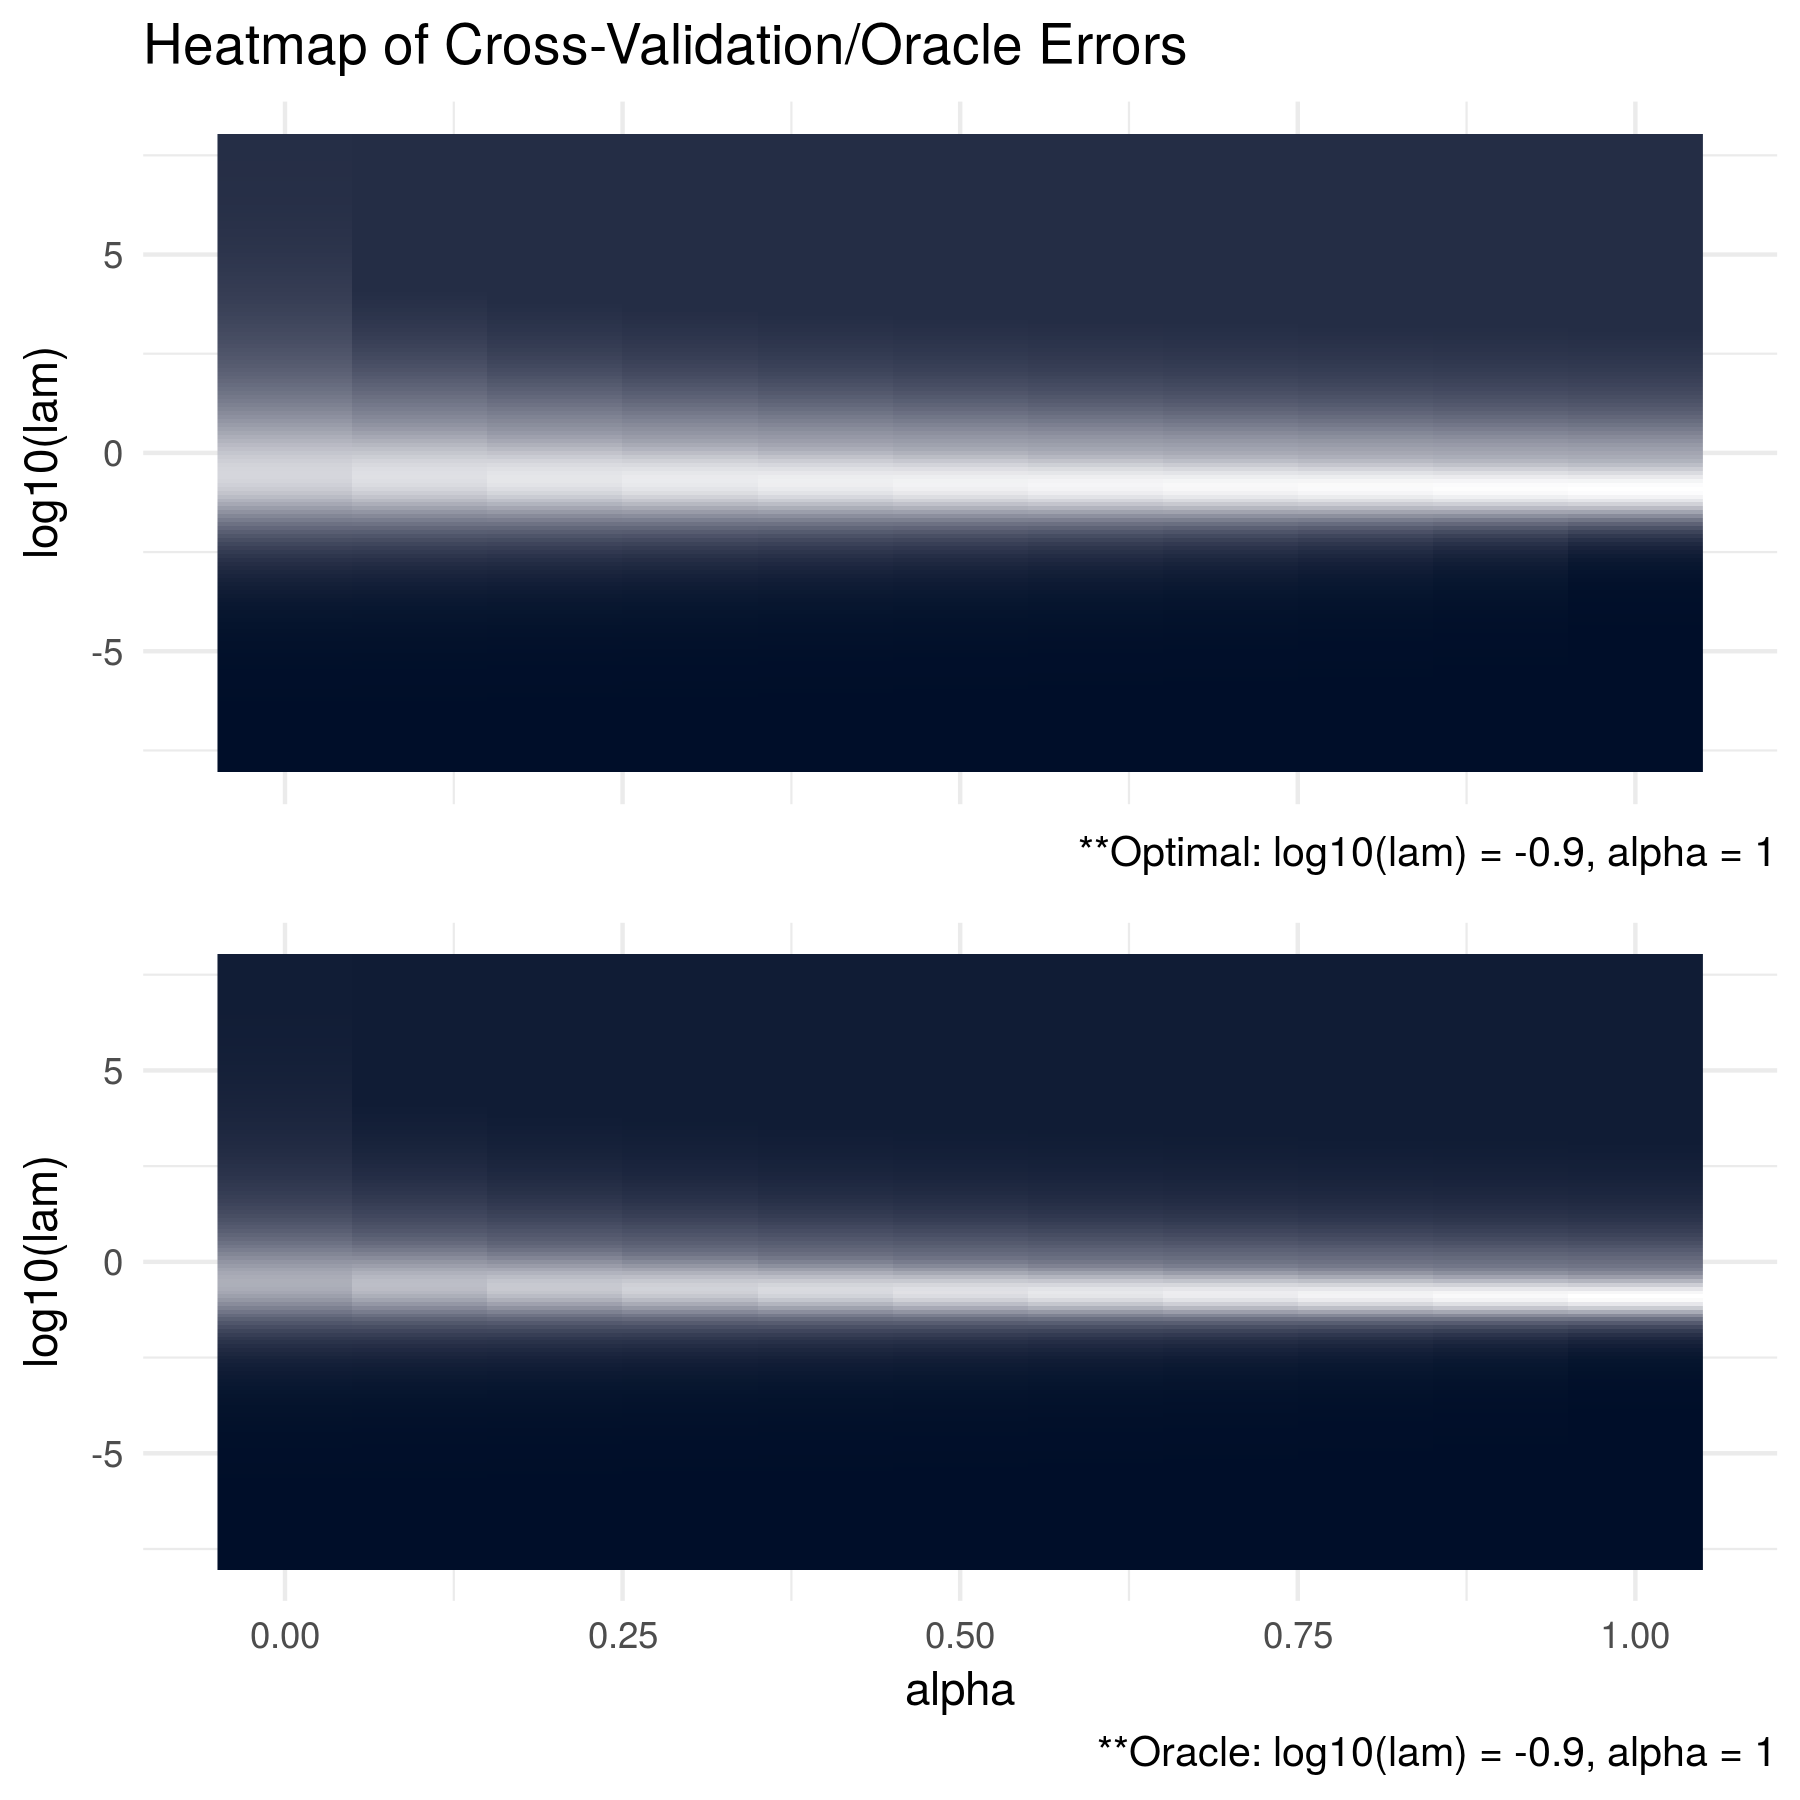
\includegraphics[width=0.85\linewidth,]{images/repsKLtridiag_N50_P100} 

}

\caption{The oracle precision matrices were tri-diagonal with dimension p = 100 and the data was generated with a sample size of n = 50. The cross validation errors are in the top figure and the KL losses between the estimated matrices and the oracle matrices are shown in the bottom figure. The optimal tuning parameter pair for each heatmap was found to be log10(lam) = -0.9 and alpha = 1. Note that brighter areas signify smaller losses.}\label{fig:admmsim5}
\end{figure}

\begin{figure}

{\centering 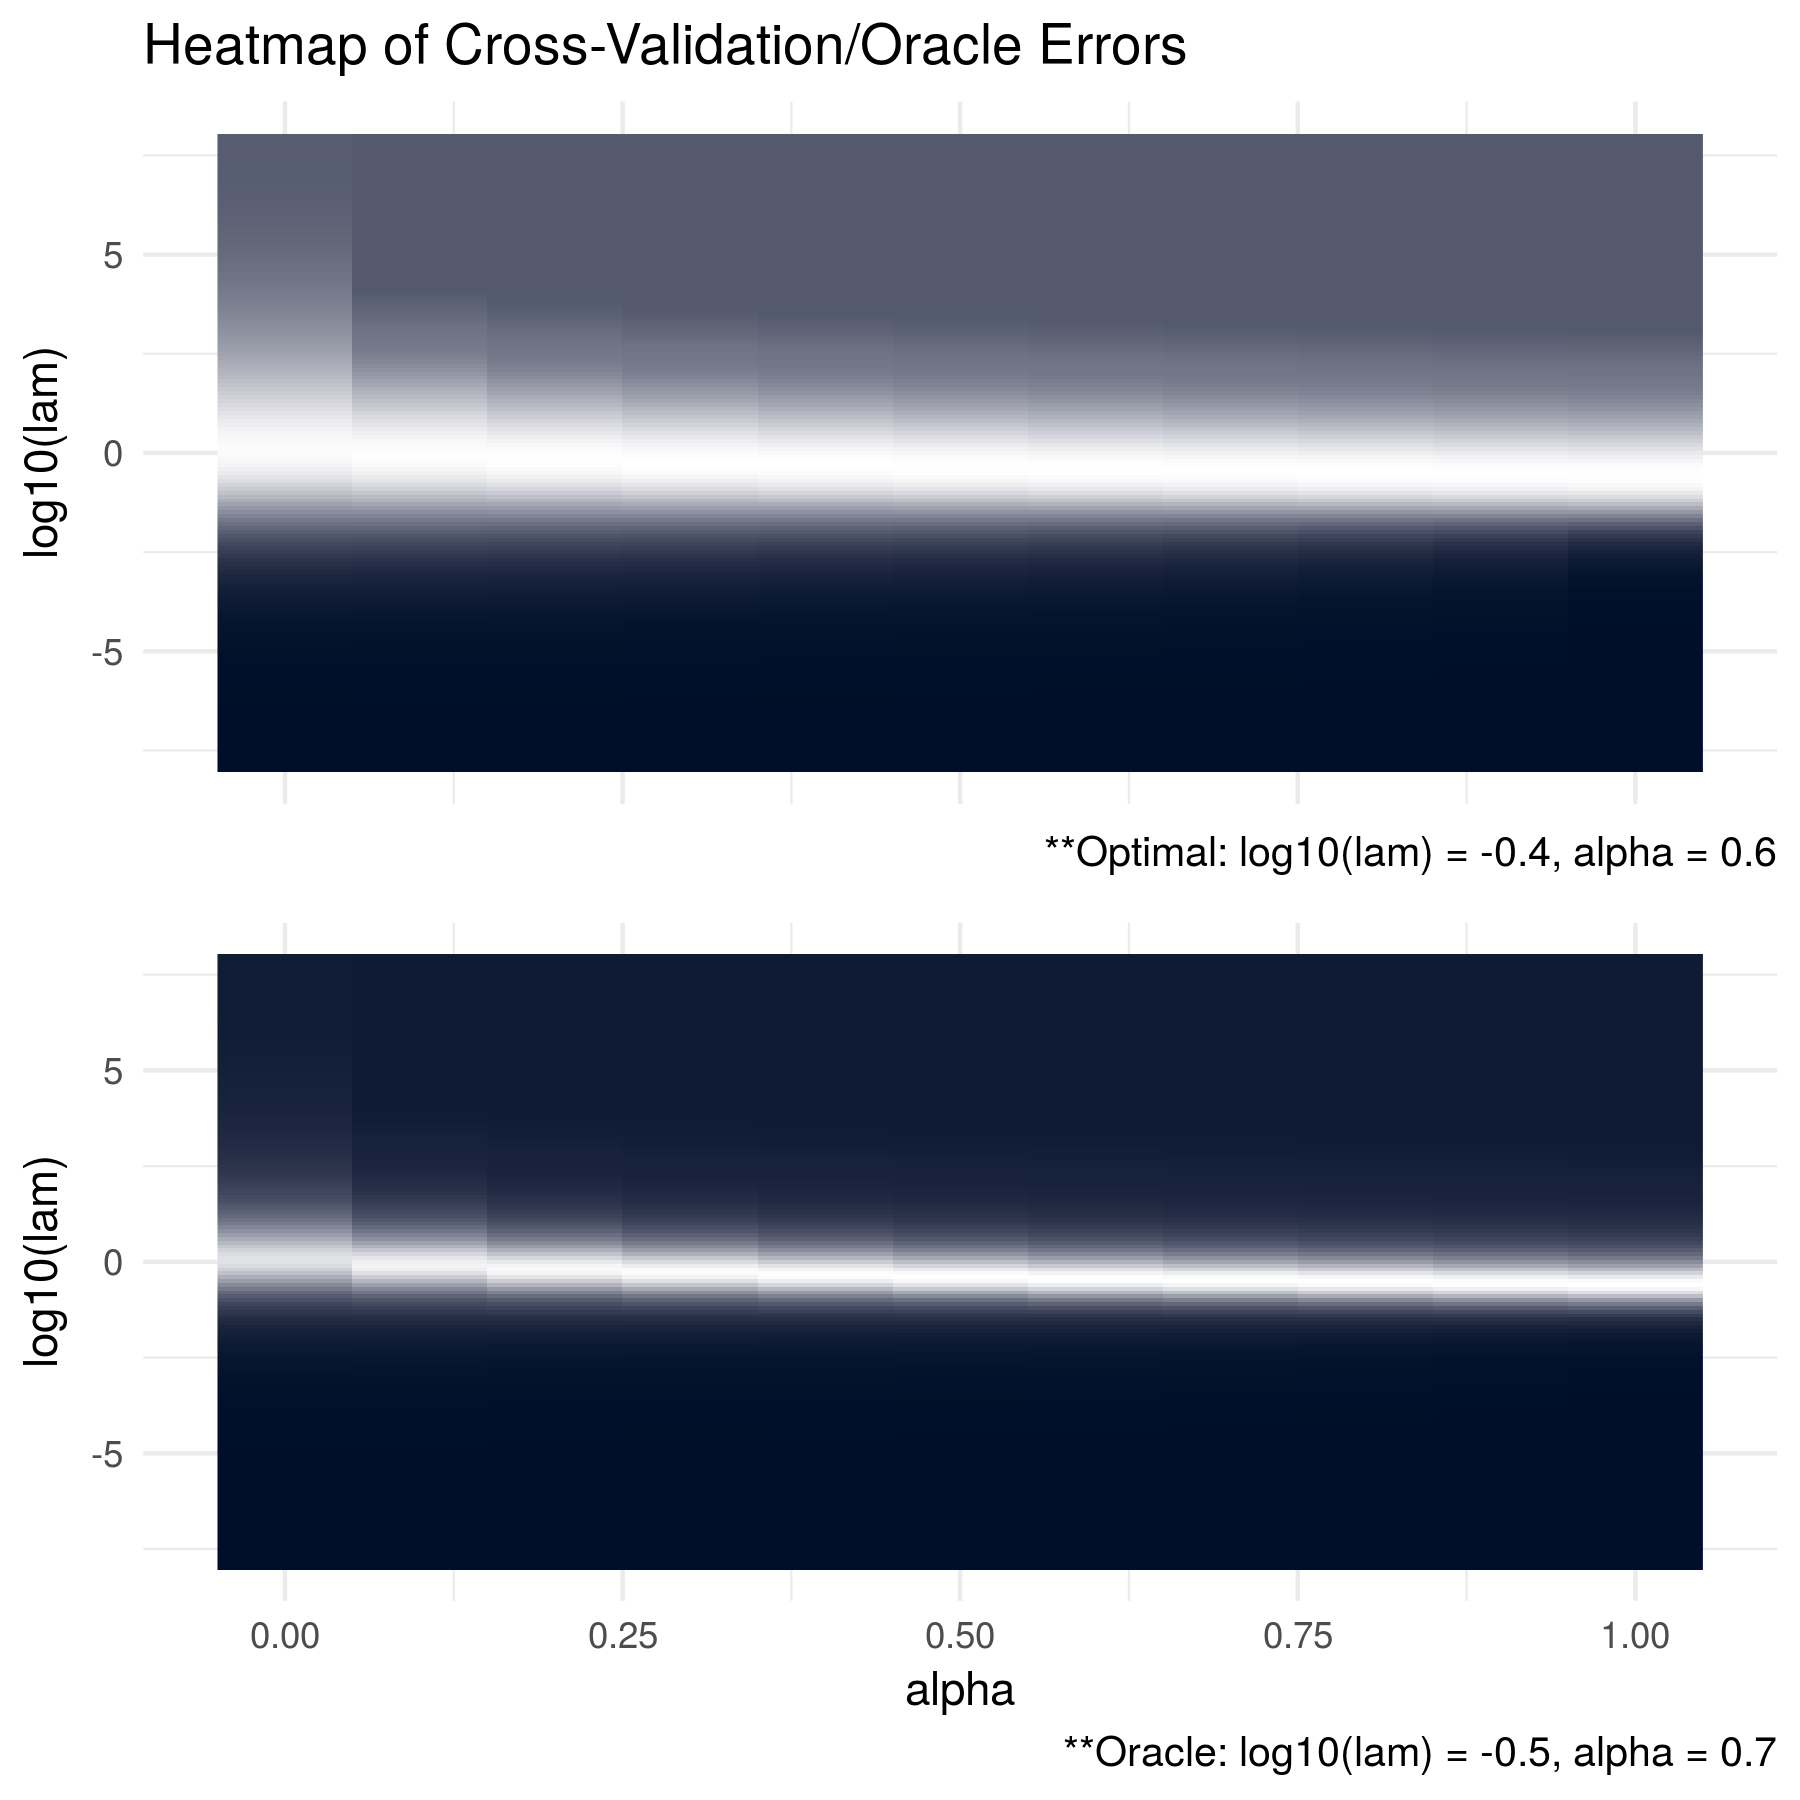
\includegraphics[width=0.85\linewidth,]{images/repsKLdenseQR_N50_P100} 

}

\caption{The oracle precision matrices were dense with dimension p = 100 and the data was generated with a sample size of n = 50. The cross validation errors are in the top figure and the KL losses between the estimated matrices and the oracle matrices are shown in the bottom figure. The optimal tuning parameter pair for the cross validation errors was found to be log10(lam) = -0.4 and alpha = 0.6 and log10(lam) = -0.5 and alpha = 0.7 for the KL losses. Note that brighter areas signify smaller losses.}\label{fig:admmsim3}
\end{figure}

\hypertarget{scpme}{%
\chapter{SCPME}\label{scpme}}

In their 2017 paper, titled \emph{Shrinking Characteristics of Precision Matrix Estimators}, Aaron Molstad, Ph.D.~and Professor Adam Rothman outline a framework to shrink a \emph{characteristic} of a precision matrix. This concept, inspired by others like \citet{cai2011direct}, \citet{fan2012road}, and \citet{mai2012direct}, exploits the fact that in many predictive models estimation of the precision matrix is only necessary through its product with another feature, such as a mean vector. The example they offer in \citet{molstad2017shrinking} is in the context of Fisher's linear discriminant analysis model. If a response vector \(Y\) is categorical such that \(Y\) can take values in \(\left\{1, ..., J\right\}\), then the linear discrimnant analysis model assumes that the design matrix \(X\) conditional on the response vector \(Y\) is normally distributed:

\begin{equation}
X | Y = j \sim N_{p}\left(\mu_{j}, \Omega^{-1}\right)
\label{eq:lda}
\end{equation}

for each \(j = 1, ..., J\). One can see from this formulation that clearly an estimation of both \(\mu\) and \(\Omega\) are required for this model. However, they note that if prediction is the primary concern, then for a given observation \(X_{i}\) only the \emph{characteristic} \(\Omega\left(\mu_{l} - \mu_{m}\right)\) is needed to discern between response categories \(l\) and \(m\). In other words, prediction only requires the characteristic \(\Omega\left(\mu_{l} - \mu_{m}\right)\) for each \(l, m \in \left\{1, ..., J\right\}\) and does \emph{not} require estimation of the full precision matrix \(\Omega\). \citet{cai2011direct} were among the first authors to propose estimating this characteristic directly but the interesting facet that distinguishes Molstad and Rothman's approach is that their framework simultaneously fits the model in \eqref{eq:lda} and performs variable selection.

The general framework has applications outside of linear discriminant analysis and we will be exploring a regression application in later sections, but first we will outline their approach. The penalty proposed by \citet{molstad2017shrinking} is of the form

\begin{equation}
P\left(\Omega\right) = \lambda\left\| A\Omega B - C \right\|_{1}
\label{eq:pen2}
\end{equation}

where \(A \in \mathbb{R}^{m \times p}, B \in \mathbb{R}^{p \times q}, \mbox{ and } C \in \mathbb{R}^{m \times q}\) are matrices that are assumed to be known and specified so that solving the full penalized gaussian negative log-likelihood for \(\Omega\) results in solving

\begin{equation}
\hat{\Omega} = \arg\min_{\Omega \in S_{+}^{p}}\left\{ tr\left(S\Omega\right) - \log\left|\Omega \right| + \lambda\left\| A\Omega B - C \right\|_{1} \right\}
\label{eq:omegaloglik2}
\end{equation}

A similar estimator was proposed by \citet{dalal2017sparse} when \(C = 0\) but here we do not require it. This form of penalty is particularly useful because it is extremely general. Note that by letting matrices \(A = I_{p}, B = I_{p}, \mbox{ and } C = 0\), this penalty reduces to a lasso penalty - but clearly this form allows for much more creative penalties and \(A, B, \mbox{ and } C\) can be constructed so that we penalize the sum, absolute value of \emph{many} characteristics of the precision matrix \(\Omega\). We will explore how to solve for \(\hat{\Omega}\) in \eqref{eq:omegaloglik2} in the next section.

\hypertarget{augmented-admm-algorithm}{%
\section{Augmented ADMM Algorithm}\label{augmented-admm-algorithm}}

Solving for \(\hat{\Omega}\) in \eqref{eq:omegaloglik2} uses what we are going to call an \emph{augmented ADMM algorithm}. Molstad and Rothman do not offer a name for this specific algorithm but it leverages the majorize-minimize principle in one of the steps in the algorithm - augmenting the original ADMM algorithm discussed in the previous chapter. Within the context of the proposed penalty, the original ADMM algorithm for precision matrix estimation would consist of iterating over the following three steps:

\begin{equation}
\begin{split}
  \Omega^{k + 1} &= \arg\min_{\Omega \in \mathbb{S}_{+}^{p}}L_{\rho}(\Omega, Z^{k}, \Lambda^{k}) \\
  Z^{k + 1} &= \arg\min_{Z \in \mathbb{R}^{n \times r}}L_{\rho}(\Omega^{k + 1}, Z, \Lambda^{k}) \\
  \Lambda^{k + 1} &= \Lambda^{k} + \rho\left(A\Omega^{k + 1}B - Z^{k + 1} - C \right)
\end{split}
\label{eq:augmentedprecision}
\end{equation}

where \(L\), the augmented lagrangian, is defined as

\begin{equation}
L_{\rho}(\Omega, Z, \Lambda) = f\left(\Omega\right) + g\left(Z\right) + tr\left[\Lambda '\left(A\Omega B - Z - C\right)\right] + \frac{\rho}{2}\left\|A\Omega B - Z - C\right\|_{F}^{2}
\label{eq:auglagrange3}
\end{equation}

Similar to the previous chapter, \(f\left(\Omega\right) = tr\left(S\Omega\right) - \log\left|\Omega\right|\) and \(g\left(Z\right) = \lambda\left\|Z\right\|_{1}\). In fact, the details of the algorithm thus far are identical to the previous approach except that we are replacing \(\Omega - Z\) with \(A\Omega B - Z - C\) in the augmented lagrangian and the dual update \(\Lambda^{k + 1}\).

Instead of solving the first step directly, the authors propose an alternative, approximating objective function, which we will denote as \(\tilde{L}\), that is based on the majorize-minimize principle\footnote{Further explanation of the majorizing function \eqref{eq:approx} in section \ref{taylorsexp}}. The purpose of this approximating function is the desire to solve the first step of the algorithm in closed-form. The ADMM algorithm with this modification based on majorize-minimize principle is also found in \citet{lange2016mm} but here we define the approximating function as

\begin{equation}
\begin{split}
  \tilde{L}_{\rho}\left(\Omega, Z^{k}, \Lambda^{k}\right) = f\left(\Omega\right) &+ g\left(Z^{k}\right) + tr\left[(\Lambda^{k})'(A\Omega B - Z^{k} - C) \right] + \frac{\rho}{2}\left\|A\Omega B - Z^{k} - C \right\|_{F}^{2} \\
  &+ \frac{\rho}{2}vec\left(\Omega - \Omega^{k}\right)' Q\left(\Omega - \Omega^{k}\right)
\end{split}
\label{eq:approx}
\end{equation}

where \(Q = \tau I_{p} - \left(A'A \otimes BB'\right)\) and \(\tau\) is chosen such that \(Q\) is positive definite. Note that if \(Q\) is positive definite, then \(L_{\rho}\left(\cdot\right) \leq \tilde{L}\left(\cdot\right)\) for all \(\Omega\) and \(\tilde{L}\) is a majorizing function\footnote{If \(Q\) is positive definite, then \(vec\left(\Omega - \Omega^{k} \right)'\rho Q\left(\Omega - \Omega^{k} \right)/2 > 0\) since \(\rho > 0\) and \(vec\left(\Omega - \Omega^{k}\right)\) is always nonzero whenever \(\Omega \neq \Omega^{k}\).}. The \emph{augmented ADMM} algorithm developed by Molstad and Rothman, which now includes the majorize-minimize principle, consists of the following repeated iterations:

\begin{equation}
\begin{split}
  \Omega^{k + 1} &= \arg\min_{\Omega \in \mathbb{S}_{+}^{p}}\left\{tr\left[\left(S + G^{k}\right)\Omega\right] - \log\left|\Omega\right| + \frac{\rho\tau}{2}\left\|\Omega - \Omega^{k}\right\|_{F}^{2} \right\}\\
  Z^{k + 1} &= \arg\min_{Z \in \mathbb{R}^{n \times r}}\left\{\lambda\left\|Z\right\|_{1} + tr\left[(\Lambda^{k})'(A\Omega B - Z^{k} - C) \right] + \frac{\rho}{2}\left\|A\Omega B - Z^{k} - C \right\|_{F}^{2} \right\} \\
  \Lambda^{k + 1} &= \Lambda^{k} + \rho\left(A\Omega^{k + 1}B - Z^{k + 1} - C \right)
\end{split}
\label{eq:augADMM}\notag
\end{equation}

where \(G^{k} = \rho A'\left( A\Omega^{k} B - Z^{k} - C + \rho^{-1}\Lambda^{k} \right)B'\). Each step in this algorithm can now conveniently be solved in closed-form and the full details of each can be found in the appendix \ref{proofOmegak}. The following theorem provides the simplified steps in the algorithm.

\BeginKnitrBlock{theorem}[Augmented ADMM Algorithm for Shrinking Characteristics of Precision Matrix Estimators.]
\protect\hypertarget{thm:unnamed-chunk-3}{}{\label{thm:unnamed-chunk-3} \iffalse (Augmented ADMM Algorithm for Shrinking Characteristics of Precision Matrix Estimators.) \fi{} }
Define the soft-thresholding function as \(\mbox{soft}(a, b) = \mbox{sign}(a)(\left| a \right| - b)_{+}\) and \(S\) as the sample covariance matrix. Set \(k = 0\) and initialize \(Z^{0}, \Lambda^{0}, \Omega^{0}\), and \(\rho\) and repeat steps 1-5 until convergence.

\begin{enumerate}
\def\labelenumi{\arabic{enumi}.}
\tightlist
\item
  Compute \(G^{k}\).
\end{enumerate}

\begin{equation}
G^{k} = \rho A'\left( A\Omega^{k} B - Z^{k} - C + \rho^{-1}\Lambda^{k} \right)B'
\label{eq:Gk}\notag
\end{equation}

\begin{enumerate}
\def\labelenumi{\arabic{enumi}.}
\setcounter{enumi}{1}
\tightlist
\item
  Via spectral decomposition, decompose
\end{enumerate}

\begin{equation}
S + \left( G^{k} + (G^{k})' \right)/2 - \rho\tau\Omega^{k} = VQV'
\label{eq:VQV}\notag
\end{equation}

\begin{enumerate}
\def\labelenumi{\arabic{enumi}.}
\setcounter{enumi}{2}
\tightlist
\item
  Update \(\Omega^{k + 1}\).\footnote{Proof of \eqref{eq:Omegak} in section \ref{proofOmegak}}
\end{enumerate}

\begin{equation}
\Omega^{k + 1} = V\left( -Q + (Q^{2} + 4\rho\tau I_{p})^{1/2} \right)V' /(2\rho\tau)
\label{eq:Omegak}
\end{equation}

\begin{enumerate}
\def\labelenumi{\arabic{enumi}.}
\setcounter{enumi}{3}
\tightlist
\item
  Update \(Z^{k + 1}\) with element-wise soft-thresholding for the resulting matrix.\footnote{Proof of \eqref{eq:Zk} in section \ref{proofZk}}
\end{enumerate}

\begin{equation}
Z^{k + 1} = \mbox{soft}\left( A\Omega^{k + 1}B - C + \rho^{-1}\Lambda^{k}, \rho^{-1}\lambda \right)
\label{eq:Zk}
\end{equation}

\begin{enumerate}
\def\labelenumi{\arabic{enumi}.}
\setcounter{enumi}{4}
\tightlist
\item
  Update \(\Lambda^{k + 1}\).
\end{enumerate}

\begin{equation}
\Lambda^{k + 1} = \Lambda^{k} + \rho\left( A\Omega^{k + 1} B - Z^{k + 1} - C \right)
\label{eq:Yk}\notag
\end{equation}
\EndKnitrBlock{theorem}

\hypertarget{stopping-criterion}{%
\subsection{Stopping Criterion}\label{stopping-criterion}}

A possibe stopping criterion for this framework is one derived from similar optimality conditions used in the previous chapter in section \ref{ADMMstop}. The primal optimality condition here is that \(A\Omega^{k + 1}B - Z^{k + 1} - C = 0\) and the two dual optimality conditions are \(0 \in \partial f\left(\Omega^{k + 1}\right) + \left(B(\Lambda^{k + 1})'A + A'\Lambda^{k + 1}B' \right)/2\) and \(0 \in \partial g\left(Z^{k + 1}\right) - \Lambda^{k + 1}\). Similarly, we will define the left-hand side of the primal optimality condition as the primal residual \(r^{k + 1} = A\Omega^{k + 1}B - Z^{k + 1} - C\) and the dual residual\footnote{Proof of \eqref{eq:stopproof} in section \ref{proofstopproof}.} as

\begin{equation}
s^{k + 1} = \frac{\rho}{2}\left( B(Z^{k + 1} - Z^{k})'A + A'(Z^{k + 1} - Z^{k})B' \right)
\label{eq:stopproof}\notag
\end{equation}

For proper convergence, we will require that both residuals are approximately equal to zero. Similar to the stopping criterion discussed previously, one possibility is to set \(\epsilon^{rel} = \epsilon^{abs} = 10^{-3}\) and stop the algorithm when \(\epsilon^{pri} \leq \left\| r^{k + 1} \right\|_{F}\) and \(\epsilon^{dual} \leq \left\| s^{k + 1} \right\|_{F}\) where

\begin{equation}
\begin{split}
  \epsilon^{pri} &= \sqrt{nr}\epsilon^{abs} + \epsilon^{rel}\max\left\{ \left\| A\Omega^{k + 1}B \right\|_{F}, \left\| Z^{k + 1} \right\|_{F}, \left\| C \right\|_{F} \right\} \\
  \epsilon^{dual} &= p\epsilon^{abs} + \epsilon^{rel}\left\| \left( B(\Lambda^{k + 1})'A + A'\Lambda^{k + 1}B' \right)/2 \right\|_{F}
\end{split}
\label{eq:scpmestopping}\notag
\end{equation}

\hypertarget{regression-illustration}{%
\section{Regression Illustration}\label{regression-illustration}}

One of the research directions mentioned in \citet{molstad2017shrinking} that was not further explored was the application of the SCPME framework to regression. Utilizing the fact that the population regression coefficient matrix \(\beta \equiv \Omega_{x}\Sigma_{xy}\) for predictors, \(X\), and the responses, \(Y\), they point out that their framework could allow for the simultaneous estimation of \(\beta\) and \(\Omega_{x}\). Like \citet{witten2009covariance}, this approach would estimate the forward regression coefficient matrix while using shrinkage estimators for the marginal population precision matrix for the predictors. For example, recall that the general optimization problem outlined in the SCPME framework is to estimate \(\hat{\Omega}\) such that

\begin{equation}
  \hat{\Omega} = \arg\min_{\Omega \in \mathbb{S}_{+}^{p}}\left\{ tr(S\Omega) - \log\left| \Omega \right| + \lambda\left\| A\Omega B - C \right\|_{1} \right\}
\label{eq:penloglik3}\notag
\end{equation}

If the user specifies that \(A = I_{p}, B = \Sigma_{xy}, C = 0, \mbox{ and } \Omega_{x}\) is the precision matrix for the predictors, then the optimization problem of interest is now

\begin{equation}
  \hat{\Omega}_{x} = \arg\min_{\Omega_{x} \in \mathbb{S}_{+}^{p}}\left\{ tr(S_{x}\Omega_{x}) - \log\left| \Omega_{x} \right| + \lambda\left\| \Omega_{x} \Sigma_{xy} \right\|_{1} \right\} \\
\label{eq:penloglik4}\notag
\end{equation}

Specifically, this optimization problem has the effect of deriving an estimate of \(\Omega_{x}\) while assuming sparsity in the forward regression coefficient \(\beta\). Of course, in practice we do not know the true covariance matrix \(\Sigma_{xy}\) but we might consider using the sample estimate \(\hat{\Sigma}_{xy} = \sum_{i = 1}^{n}\left(X_{i} - \bar{X}\right)\left(Y_{i} - \bar{Y}\right)'/n\) in place of \(\Sigma_{xy}\). We could then use our estimator, \(\hat{\Omega}_{x}\), to construct the estimated forward regression coefficient matrix \(\hat{\beta} = \hat{\Omega}_{x}\hat{\Sigma}_{xy}\). Estimators such as these are truly novel an can conveniently be estimated by the SCPME framework. Another such estimator that is a product of this new framework is one where we construct \(A \mbox{ and } C\) similarly but take \(B = \left[ \Sigma_{xy}, I_{p} \right]\) so that the identity matrix is appended to the cross-covariance matrix of \(X\) and \(Y\). In this case, not only are we assuming that \(\beta\) is sparse, but we are also assuming sparsity in \(\Omega\).

\begin{equation}
P_{\lambda}\left(\Omega \right) = \lambda\left\| A\Omega B - C \right\|_{1} = \lambda\left\| \Omega\left[\Sigma_{xy}, I_{p}\right] \right\|_{1} = \lambda\left\| \beta \right\|_{1} + \lambda\left\| \Omega \right\|_{1}
\label{eq:pen4}\notag
\end{equation}

Like before, we could use \(\hat{\Sigma}_{xy}\) as a replacement and take our resulting estimator, \(\hat{\Omega}_{x}\), to construct the estimated forward regression coefficient matrix \(\hat{\beta} = \hat{\Omega}_{x}\hat{\Sigma}_{xy}\). The embedded assumptions here are that not all predictors in \(X\) are useful in predicting the response, \(Y\), \emph{and} that a number of the predictors are conditionally independent of one another. These are assumptions that are quite reasonable in practice and in the next section we offer a short simulation comparing these new estimators to related and competing prediction methods.

\hypertarget{simulations-1}{%
\section{Simulations}\label{simulations-1}}

In this simulation, we compare, under various data realizations, the performance of several competing regression prediction methods including the new so-called SCPME regression estimators discussed in the previous section. In total, we consider the following:

\begin{itemize}
\item
  \texttt{OLS} = ordinary least squares estimatior. In high dimensional settings (\(p >> n\)), the Moore-Penrose estimator is used as a replacement.
\item
  \texttt{ridge} = ridge regression estimator.
\item
  \texttt{lasso} = lasso regression estimator.
\item
  \texttt{oracleB} = oracle estimator for \(\beta\).
\item
  \texttt{oracleO} = regression estimator with oracle \(\Omega_{x}^{*}\) (let \(\beta = \Omega_{x}^{*}\hat{\Sigma}_{xy}\)).
\item
  \texttt{oracleS} = regression estimator with oracle \(\Sigma_{xy}^{*}\) (let \(\beta = \hat{\Omega}_{x}\Sigma_{xy}^{*}\)) and \(\Omega_{x}\) is estimated using an elastic-net penalty.
\item
  \texttt{shrinkB} = SCPME regression estimator with penalty \(\lambda\left\| \Omega_{x}\hat{\Sigma}_{xy} \right\|_{1}\) so that \(\beta = \hat{\Omega}_{x}\hat{\Sigma}_{xy}\).
\item
  \texttt{shrinkBS} = SCPME regression estimator with oracle \(\Sigma_{xy}^{*}\) so that the penalty is \(\lambda\left\| \Omega_{x}\Sigma_{xy}^{*} \right\|_{1}\) and we let \(\beta = \hat{\Omega}_{x}\Sigma_{xy}^{*}\).
\item
  \texttt{shrinkBO} = SCPME regression estimator with penalty \(\lambda\left\| \Omega_{x}[\hat{\Sigma}_{xy}, I_{p}] \right\|_{1}\) so that \(\beta = \hat{\Omega}_{x}\hat{\Sigma}_{xy}\).
\item
  \texttt{glasso} = graphical lasso estimator with penalty \(\lambda\left\| \Omega_{x} \right\|_{1}\) so that \(\beta = \hat{\Omega}_{x}\hat{\Sigma}_{xy}\).
\end{itemize}

For each estimator, if selection of a tuning parameter is required, the tuning parameter was chosen so that the mean squared prediction error (MSPE) was minimized over 3-fold cross validation.

The data generating procedure for the simulations is the following. The oracle regression coefficient matrix \(\beta^{*}\) was constructed so that \(\beta^{*} = \mathbb{B} \circ \mathbb{V}\) where \(vec\left( \mathbb{B} \right) \sim N_{pr}\left( 0, I_{p} \otimes I_{r}/\sqrt{p} \right)\) and \(\mathbb{V} \in \mathbb{R}^{p \times r}\) is a matrix containing \(p\) times \(r\) random bernoulli draws with 50\% probability being equal to one. The covariance matrices \(\Sigma_{y | x}\) and \(\Sigma_{x}\) were constructed so that \(\left( \Sigma_{y | x} \right)_{ij} = 0.7^{\left| i - j \right|}\) and \(\left( \Sigma_{x} \right)_{ij} = 0.7^{\left| i - j \right|}\), respectively. This ensures that their corresponding precision matrices will be tridiagonal and sparse. Then for 100 independent, identically distributed samples, we had \(X_{i} \sim N_{p}\left( 0, \Sigma_{x} \right)\) and \(E_{i} \sim N_{r}\left( 0, \Sigma_{y | x} \right)\) so that \(\mathbb{Y} = \mathbb{X}\beta + \mathbb{E}\) where \(\mathbb{X} \in \mathbb{R}^{n \times p}\) and \(\mathbb{Y} \in \mathbb{R}^{n \times r}\) are the matrices with stacked rows \(X_{i}\) and \(E_{i}\), respectively, for \(i = 1, ..., n\) and the script notation denotes the fact that the columns have been centered so as to remove the intercept in our prediction models. A sample of an additional 1000 observations was generated similarly for the testing set. Each prediction method was evaluated on both model error and mean squared prediction error.

Figure \ref{fig:scpmesim2} displays the model error for each method by dimension of the design matrix. Here we took the sample size equal to \(n = 100\) and the response matrix dimension \(r = 10\) with each data generating procedure replicated a total of 20 times. Note \texttt{OLS} and \texttt{oracleS} are not shown due to extremely poor performance. We find that in high dimensional settings, \texttt{shrinkBO} and \texttt{shrinkB} perform increasingly well relative to the others as the predictor dimension increases. \texttt{shrinkBO} performed the best. Interestingly, when \(n > p\) \texttt{shrinkBO} is still one of the best-performing estimators - though worse than both \texttt{lasso} and \texttt{ridge} - but the performance of \texttt{shrinkB} decreases drastically (plot not shown).

In the high dimension setting, the oracle estimators \texttt{oracleO} and \texttt{oracleS} performed worse or comparable to the \texttt{OLS} estimator. The poor performance of \texttt{oracleS} is likely due to the fact that the sample estimate of \(\Omega_{x}\) is not identifiable when \(p > n\).

The following table shows the average model error for each estimator when \(n = 100\), \(p = 150\), and \(r = 10\).

\vspace{0.5cm}
\begin{figure}

{\centering 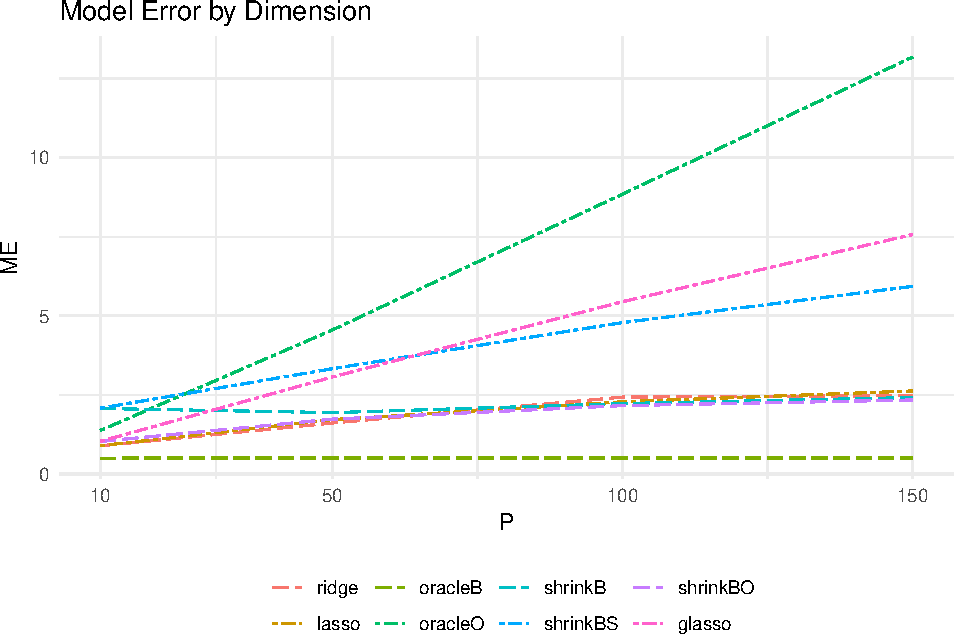
\includegraphics[width=0.85\linewidth,]{Manuscript_files/figure-latex/scpmesim2-1} 

}

\caption{The oracle precision matrices were tri-diagonal with variable dimension (p) and the data was generated with sample size n = 100 and response vector dimension r = 10. The model errors (ME) for each estimator with variable dimension of the design matrix are plotted. shrinkBO and shrinkB were the two best-performing estimators closely follow by the ridge and lasso regression estimators.}\label{fig:scpmesim2}
\end{figure}

\newpage

\begin{longtable}[]{@{}ccc@{}}
\caption{Average model error for dimension p = 150.
\vspace{0.5cm}}\tabularnewline
\toprule
\begin{minipage}[b]{0.14\columnwidth}\centering
Model\strut
\end{minipage} & \begin{minipage}[b]{0.11\columnwidth}\centering
Error\strut
\end{minipage} & \begin{minipage}[b]{0.11\columnwidth}\centering
SD\strut
\end{minipage}\tabularnewline
\midrule
\endfirsthead
\toprule
\begin{minipage}[b]{0.14\columnwidth}\centering
Model\strut
\end{minipage} & \begin{minipage}[b]{0.11\columnwidth}\centering
Error\strut
\end{minipage} & \begin{minipage}[b]{0.11\columnwidth}\centering
SD\strut
\end{minipage}\tabularnewline
\midrule
\endhead
\begin{minipage}[t]{0.14\columnwidth}\centering
oracleB\strut
\end{minipage} & \begin{minipage}[t]{0.11\columnwidth}\centering
0.5056\strut
\end{minipage} & \begin{minipage}[t]{0.11\columnwidth}\centering
0.5122\strut
\end{minipage}\tabularnewline
\begin{minipage}[t]{0.14\columnwidth}\centering
shrinkBO\strut
\end{minipage} & \begin{minipage}[t]{0.11\columnwidth}\centering
2.341\strut
\end{minipage} & \begin{minipage}[t]{0.11\columnwidth}\centering
1.014\strut
\end{minipage}\tabularnewline
\begin{minipage}[t]{0.14\columnwidth}\centering
shrinkB\strut
\end{minipage} & \begin{minipage}[t]{0.11\columnwidth}\centering
2.419\strut
\end{minipage} & \begin{minipage}[t]{0.11\columnwidth}\centering
1.083\strut
\end{minipage}\tabularnewline
\begin{minipage}[t]{0.14\columnwidth}\centering
ridge\strut
\end{minipage} & \begin{minipage}[t]{0.11\columnwidth}\centering
2.479\strut
\end{minipage} & \begin{minipage}[t]{0.11\columnwidth}\centering
1.128\strut
\end{minipage}\tabularnewline
\begin{minipage}[t]{0.14\columnwidth}\centering
lasso\strut
\end{minipage} & \begin{minipage}[t]{0.11\columnwidth}\centering
2.627\strut
\end{minipage} & \begin{minipage}[t]{0.11\columnwidth}\centering
1.27\strut
\end{minipage}\tabularnewline
\begin{minipage}[t]{0.14\columnwidth}\centering
shrinkBS\strut
\end{minipage} & \begin{minipage}[t]{0.11\columnwidth}\centering
5.932\strut
\end{minipage} & \begin{minipage}[t]{0.11\columnwidth}\centering
4.001\strut
\end{minipage}\tabularnewline
\begin{minipage}[t]{0.14\columnwidth}\centering
glasso\strut
\end{minipage} & \begin{minipage}[t]{0.11\columnwidth}\centering
7.57\strut
\end{minipage} & \begin{minipage}[t]{0.11\columnwidth}\centering
5.412\strut
\end{minipage}\tabularnewline
\begin{minipage}[t]{0.14\columnwidth}\centering
oracleO\strut
\end{minipage} & \begin{minipage}[t]{0.11\columnwidth}\centering
13.18\strut
\end{minipage} & \begin{minipage}[t]{0.11\columnwidth}\centering
10.11\strut
\end{minipage}\tabularnewline
\begin{minipage}[t]{0.14\columnwidth}\centering
OLS\strut
\end{minipage} & \begin{minipage}[t]{0.11\columnwidth}\centering
14.41\strut
\end{minipage} & \begin{minipage}[t]{0.11\columnwidth}\centering
11.24\strut
\end{minipage}\tabularnewline
\begin{minipage}[t]{0.14\columnwidth}\centering
oracleS\strut
\end{minipage} & \begin{minipage}[t]{0.11\columnwidth}\centering
52.07\strut
\end{minipage} & \begin{minipage}[t]{0.11\columnwidth}\centering
44.62\strut
\end{minipage}\tabularnewline
\bottomrule
\end{longtable}

\hypertarget{regression-simulations-with-covariance-shrinkage}{%
\subsection{Regression Simulations with Covariance Shrinkage}\label{regression-simulations-with-covariance-shrinkage}}

This final simulation was explored due to the fact that each of the SCPME regression estimators require an estimation of the cross-covariance matrix. In the previous simulations, we naively used the maximum likelihood estimate. However, because the data-generating procedure constructs settings that are inherently sparse, we were interested to determine if additional shrinkage of the maximum likelihood estimate for the \emph{cross-covariance} matrix would also prove beneficial. For instance, in a number of settings, we were finding that the estimator \texttt{oracleO} was performing worse than \texttt{oracleS}. This perhaps suggests that estimating the covariance matrix \(\Sigma_{xy}\) well is \emph{more} important than estimating \(\Omega\) well. This simulation explores that theory a bit further.

The data-generating procedure for this simulation is similar to previous one but here we take \(n = 100\), \(p = 200\), \(r = 10\), and, in addition, we multiply the population cross-covariance estimator by a factor of \(k\) where \(k \in (0.1, 0.2, ..., 0.9, 1)\). Figure \ref{fig:scpmesim7} plots the MSPE for \texttt{shrinkB} for each tuning parameter, \(\lambda\), and constant, \(k\), pair. Figure \ref{fig:scpmesim9} plots the MSPE similarly for \texttt{shrinkBO}.

Interestingly, we find that in this high dimension setting, it does appear that shrinking the sample covariance matrix by a constant factor helps the overall prediction performance of the SCPME estimators. This is indicated by the fact that the optimal constant, \(k\), hovers between 0.3 and 0.6 for each of the estimators. We also performed a simulation in low dimensions (not shown) but we did not see the same benefit.

\vspace{0.5cm}

\vspace{0.5cm}
\begin{figure}

{\centering 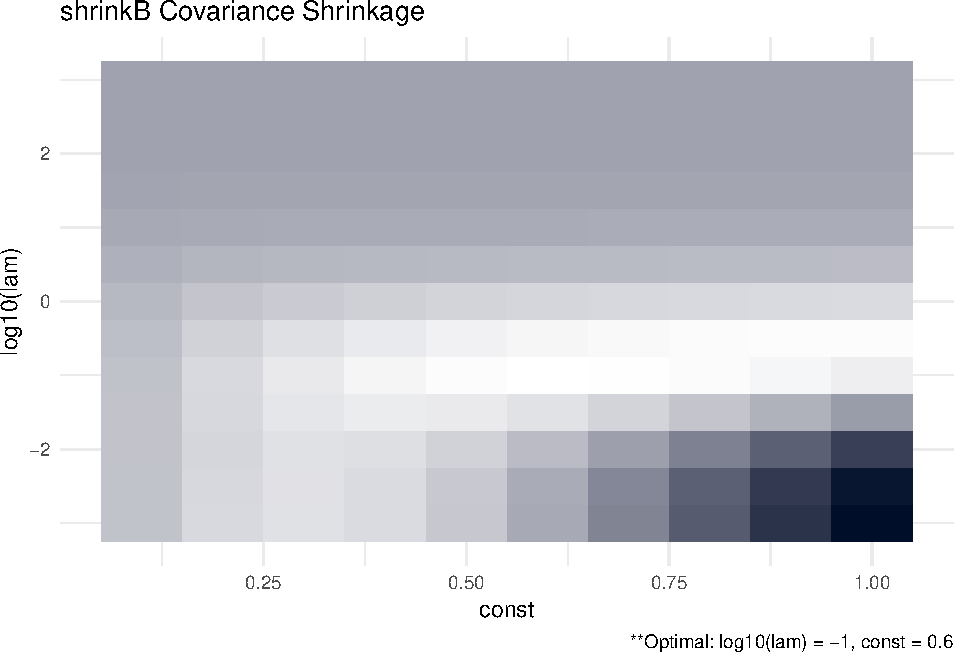
\includegraphics[width=0.85\linewidth,]{Manuscript_files/figure-latex/scpmesim7-1} 

}

\caption{The oracle precision matrices were tri-diagonal with dimension p = 200 and the data was generated with a sample size n = 100 and response vector dimension r = 10. The cross validation MSPE are plotted for each lambda and constant tuning parameter pair. The optimal tuning parameter pair was found to be log10(lam) = -1 and const = 0.6. Note that brighter areas signify smaller losses.}\label{fig:scpmesim7}
\end{figure}
\vspace{0.5cm}

\vspace{0.5cm}
\begin{figure}

{\centering 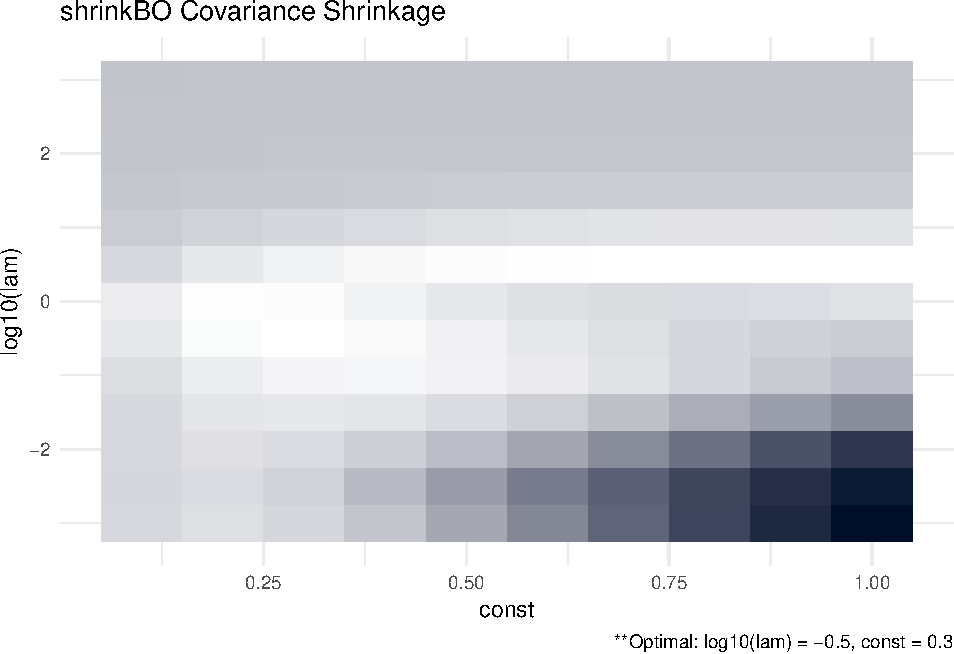
\includegraphics[width=0.85\linewidth,]{Manuscript_files/figure-latex/scpmesim9-1} 

}

\caption{The oracle precision matrices were tri-diagonal with dimension p = 200 and the data was generated with a sample size n = 100 and response vector dimension r = 10. The cross validation MSPE are plotted for each lambda and constant tuning parameter pair. The optimal tuning parameter pair was found to be log10(lam) = -0.5 and const = 0.3. Note that brighter areas signify smaller losses.}\label{fig:scpmesim9}
\end{figure}
\vspace{0.5cm}

\newpage

\hypertarget{discussion}{%
\section{Discussion}\label{discussion}}

Apart from the two SCPME estimators discussed in the previous section, the generality of the SCPME framework allows for many previously unconceptualized precision matrix estimators to be explored. One estimator that was concieved of in our work but deserves further attention in future research is of the form

\begin{equation}
\hat{\Omega}_{x} = \arg\min_{\Omega_{x} \in \mathbb{S}_{+}^{p}}\left\{ tr(S_{x}\Omega_{x}) - \log\left| \Omega_{x} \right| + \frac{\lambda}{2}\left\| \mathbb{X}\Omega_{x} \Sigma_{xy} - \mathbb{Y} \right\|_{F}^{2} \right\}
\label{eq:penregression}\notag
\end{equation}

For clarity in regards to the SCPME framework, \(A = \mathbb{X}, B = \Sigma_{xy}, \mbox{ and } C = \mathbb{Y}\). As before, \(\mathbb{X}\) is the \(n \times p\) matrix with rows \(X_{i} \in \mathbb{R}^{p}\) for \(i = 1,..., n\) and the script notation denotes that the matrix has been column-centered. The matrix \(\mathbb{Y}\) is a similar representation for the observed responses \(Y_{i} \in \mathbb{R}^{r}\). Also note that here we are using the Frobenius norm instead of the matrix \(l_{1}\)-norm but this replacement requires only a slight modification of the augmented ADMM algorithm for optimization - details of which will be presented later.

This optimization problem estimates a precision matrix that balances minimizing the gaussian negative log-likelihood for \(\Omega_{x}\) with minimizing the squared prediction error for the forward regression model. In other words, the objective function aims to penalize estimates, determined by \(\lambda\), that too heavily favor maximizing the marginal likelihood for \(X\) over the predictive performance of the conditional model \(Y\) given \(X\). This estimator also reveals an interesting connection to the joint log-likelihood of the two random variables. To see this, let us suppose that we have \(n\) independent copies of the random pair \((Y_{i}, X_{i})\) and we assume a linear relationship such that

\begin{equation}
Y_{i} = \mu_{y} + \beta'\left(X_{i} - \mu_{x}\right) + E_{i}
\end{equation}

where \(E_{i} \sim N_{r}\left( 0, \Omega_{y | x}^{-1} \right)\) and \(X_{i} \sim N_{p}\left( \mu_{x}, \Omega_{x}^{-1} \right)\). This implies that the conditional distribution of \(Y_{i}|X_{i}\) is of the form

\begin{equation}
Y_{i} | X_{i} \sim N_{r}\left( \mu_{y} + \beta'\left(X_{i} - \mu_{x}\right), \Omega_{y | x}^{-1} \right)
\end{equation}

We can use this conditional distribution along with the marginal distribution of \(X\) to derive the joint log-likelihood of \(X\) and \(Y\). Recall that \(\beta \equiv \Omega_{x}\Sigma_{xy}\) and \(S_{x}\) is the marginal sample covariance matrix of \(X\). Without loss of generality, we will assume here that \(\mu_{x} = \mu_{y} = 0\).

\begin{equation}
\begin{split}
  l\left( \Omega_{y | x}, \Omega_{x}, \Sigma_{xy} | Y, X \right) &= constant + \frac{n}{2}\log\left| \Omega_{y | x} \right| - \frac{1}{2}\sum_{i = 1}^{n} tr\left[ \left( Y_{i} - \Sigma_{xy}'\Omega_{x} X_{i} \right)\left( Y_{i} - \Sigma_{xy}'\Omega_{x} X_{i} \right)'\Omega_{y | x} \right] \\
  &+\frac{n}{2}\log\left| \Omega \right| - \frac{1}{2}\sum_{i = 1}^{n}tr\left( X_{i}X_{i}'\Omega_{x} \right) \\
  &= constant + \frac{n}{2}\log\left| \Omega_{y | x} \right| - \frac{1}{2}tr\left[ \left( \mathbb{Y} - \mathbb{X}\Omega_{x}\Sigma_{xy} \right)'\left( \mathbb{Y} - \mathbb{X}\Omega_{x}\Sigma_{y | x} \right)\Omega_{y | x} \right] \\
  &+ \frac{n}{2}\log\left| \Omega_{x} \right| - \frac{n}{2}tr\left( S_{x}\Omega_{x} \right)
\end{split}
\label{eq:partialjointloglik}\notag
\end{equation}

Optimizing this joint log-likelihood with respect to \(\Omega_{x}\) reveals strong similiarities to the estimator that was derived from the SCPME framework:

\begin{equation}
\begin{split}
  \hat{\Omega}_{x} &= \arg\min_{\Omega_{x} \in \mathbb{S}_{+}^{p}}\left\{ \frac{1}{2}tr\left[ \left( \mathbb{Y} - \mathbb{X}\Omega_{x}\Sigma_{xy} \right)'\left( \mathbb{Y} - \mathbb{X}\Omega_{x}\Sigma_{xy} \right)\Omega_{y | x} \right] + \frac{n}{2}tr\left( S_{x}\Omega_{x} \right) - \frac{n}{2}\log\left| \Omega_{x} \right| \right\} \\
  &= \arg\min_{\Omega_{x} \in \mathbb{S}_{+}^{p}}\left\{ tr\left( S_{x}\Omega_{x} \right) - \log\left| \Omega_{x} \right| + \frac{1}{n}\left\| \left( \mathbb{X}\Omega_{x}\Sigma_{xy} - \mathbb{Y} \right)\Omega_{y | x}^{1/2} \right\|_{F}^{2} \right\}
\end{split}
\label{eq:omegajointloglik}\notag
\end{equation}

If it is the case that, given \(X\), each of the \(r\) responses are pairwise independent with equal variance so that \(\Omega_{y | x}^{1/2} = \sigma_{y | x}I_{r}\) and we let \(\lambda = 2\sigma_{y | x}^{2}/n\), then we have that

\begin{equation}
\hat{\Omega}_{x} = \arg\min_{\Omega_{x} \in \mathbb{S}_{+}^{p}}\left\{ tr\left( S_{x}\Omega_{x} \right) - \log\left| \Omega_{x} \right| + \frac{\lambda}{2}\left\| \mathbb{X}\Omega_{x}\Sigma_{xy} - \mathbb{Y} \right\|_{F}^{2} \right\}
\label{eq:omegajointmle}\notag
\end{equation}

This is exactly the estimator conceived of previously. Of course, throughout this derivation there were several assumptions that were made and in practice we do not know the true values of neither \(\Omega_{y | x}\) nor \(\Sigma_{xy}\). However, we can see that this estimator is solving a very similar problem to that of optimizing the joint log-likelihood with respect to \(\Omega_{x}\). We think this estimator and related ones deserve attention in future work.

The algorithm for solving this optimization problem is below. Note that no closed-form solution exists and so we must resort to some iterative algorithm similar to the SCPME augmented ADMM algorithm\footnote{Proof in section \ref{proofpenregression}.}. The only difference here is that in step four we no longer require elementwise soft-thresholding.

\BeginKnitrBlock{theorem}[Modified Augmented ADMM Algorithm for Shrinking Characteristics of Precision Matrix Estimators with Frobenius Norm]
\protect\hypertarget{thm:unnamed-chunk-6}{}{\label{thm:unnamed-chunk-6} \iffalse (Modified Augmented ADMM Algorithm for Shrinking Characteristics of Precision Matrix Estimators with Frobenius Norm) \fi{} }
Set \(k = 0\) and initialize \(Z^{0}, \Lambda^{0}, \Omega^{0}\), and \(\rho\) and repeat steps 1-5 until convergence.

\begin{enumerate}
\def\labelenumi{\arabic{enumi}.}
\item
  Compute \(G^{k} = \rho A'\left( A\Omega^{k} B - Z^{k} - C + \rho^{-1}\Lambda^{k} \right)B'\)
\item
  Decompose \(S + \left( G^{k} + (G^{k})' \right)/2 - \rho\tau\Omega^{k} = VQV'\) (via the spectral decomposition).
\item
  Set \(\Omega^{k + 1} = V\left( -Q + (Q^{2} + 4\rho\tau I_{p})^{1/2} \right)V'/(2\rho\tau)\)
\item
  Set \(Z^{k + 1} = \left[ \rho\left( A\Omega^{k + 1} B - C \right) + \Lambda^{k} \right]/(\lambda + \rho)\)
\item
  Set \(\Lambda^{k + 1} = \rho\left( A\Omega^{k + 1} B - Z^{k + 1} - C \right)\)
\end{enumerate}
\EndKnitrBlock{theorem}

\hypertarget{appendix-appendix}{%
\appendix}


\hypertarget{appendix}{%
\chapter{Appendix}\label{appendix}}

\hypertarget{proofomegaalgo}{%
\subsection{Proof of \eqref{eq:omegaalgo}}\label{proofomegaalgo}}

\citet{witten2009covariance} and \citet{price2015ridge} showed that the following optimization problem can be solved in closed-form. We outline their steps here.

\begin{equation}
\Omega^{k + 1} = \arg\min_{\Omega \in \mathbb{S}_{+}^{p}}\left\{ tr\left(S\Omega\right) - \log\left|\Omega\right| + tr\left[\Lambda^{k}\left(\Omega - Z^{k}\right)\right] + \frac{\rho}{2}\left\| \Omega - Z^{k} \right\|_{F}^{2} \right\}
\label{eq:appendixomegaloglik}\notag
\end{equation}

First start by taking the gradient with respect to \(\Omega\):

\begin{equation}
\begin{split}
  \nabla_{\Omega}&\left\{ tr\left(S\Omega\right) - \log\left|\Omega\right| + tr\left[\Lambda^{k}\left(\Omega - Z^{k}\right)\right] + \frac{\rho}{2}\left\| \Omega - Z^{k} \right\|_{F}^{2} \right\} \\
  &= S - \Omega^{-1} + \Lambda^{k} + \rho\left( \Omega - Z^{k} \right)
\end{split}
\label{eq:appendixomegagradient}\notag
\end{equation}

Note that because all of the variables are symmetric, we can ignore the symmetric constraint when deriving the gradient. Next set the gradient equal to zero and decompose \(\Omega^{k + 1} = VDV'\) using spectral decomposition so that \(D\) is a diagonal matrix with diagonal elements equal to the eigen values of \(\Omega^{k + 1}\) and \(V\) is the matrix with corresponding eigen vectors as columns so that

\begin{equation}
S + \Lambda^{k} - \rho Z^{k} = (\Omega^{k + 1})^{-1} - \rho \Omega^{k + 1} = VD^{-1}V' - \rho VDV' =  V\left(D^{-1} - \rho D\right)V'\notag
\end{equation}

This equivalence implies that

\begin{equation}
\phi_{j}\left( S + \Lambda^{k} - \rho Z^{k} \right) = \frac{1}{\phi_{j}(\Omega^{k + 1})} - \rho\phi_{j}(\Omega^{k + 1})\notag
\end{equation}

where \(\phi_{j}(\cdot)\) is the \(j\)th eigen value.

\begin{equation}
\begin{split}
  &\Rightarrow \rho\phi_{j}^{2}(\Omega^{k + 1}) + \phi_{j}\left( S + \Lambda^{k} - \rho Z^{k} \right)\phi_{j}(\Omega^{k + 1}) - 1 = 0 \\
  &\Rightarrow \phi_{j}(\Omega^{k + 1}) = \frac{-\phi_{j}(S + \Lambda^{k} - \rho Z^{k}) \pm \sqrt{\phi_{j}^{2}(S + \Lambda^{k} - \rho Z^{k}) + 4\rho}}{2\rho}
\end{split}
\notag
\end{equation}

In summary, if we decompose \(S + \Lambda^{k} - \rho Z^{k} = VQV'\) then

\begin{equation}
\Omega^{k + 1} = \frac{1}{2\rho}V\left[ -Q + (Q^{2} + 4\rho I_{p})^{1/2}\right] V'
\label{eq:appendixomegaproof}
\end{equation}

\hypertarget{proofZZalgo}{%
\subsection{Proof of \eqref{eq:ZZalgo}}\label{proofZZalgo}}

Solve the optimization problem

\begin{equation}
Z^{k + 1} = \arg\min_{Z \in \mathbb{S}^{p}}\left\{ \lambda\left[ \frac{1 - \alpha}{2}\left\| Z \right\|_{F}^{2} + \alpha\left\| Z \right\|_{1} \right] + tr\left[\Lambda^{k}\left(\Omega^{k + 1} - Z\right)\right] + \frac{\rho}{2}\left\| \Omega^{k + 1} - Z \right\|_{F}^{2} \right\}
\label{eq:appendixZZloglik}\notag
\end{equation}

Start by taking the subgradient with respect to \(Z\):

\begin{equation}
\begin{split}
  \partial&\left\{ \lambda\left[ \frac{1 - \alpha}{2}\left\| Z \right\|_{F}^{2} + \alpha\left\| Z \right\|_{1} \right] + tr\left[\Lambda^{k}\left(\Omega^{k + 1} - Z\right)\right] + \frac{\rho}{2}\left\| \Omega^{k + 1} - Z \right\|_{F}^{2} \right\} \\
  &= \partial\left\{ \lambda\left[ \frac{1 - \alpha}{2}\left\| Z \right\|_{F}^{2} + \alpha\left\| Z \right\|_{1} \right] \right\} + \nabla_{\Omega}\left\{ tr\left[\Lambda^{k}\left(\Omega^{k + 1} - Z\right)\right] + \frac{\rho}{2}\left\| \Omega^{k + 1} - Z \right\|_{F}^{2} \right\} \\
  &= \lambda(1 - \alpha)Z + \mbox{sign}(Z)\lambda\alpha - \Lambda^{k} - \rho\left( \Omega^{k + 1} - Z \right)
\end{split}
\label{eq:appendixZZgradient}\notag
\end{equation}

where sign is the elementwise sign operator. By setting the gradient/sub-differential equal to zero, we have that

\begin{equation}
Z_{ij}^{k + 1} = \frac{1}{\lambda(1 - \alpha) + \rho}\left( \rho \Omega_{ij}^{k + 1} + \Lambda_{ij}^{k} - \mbox{sign}(Z_{ij}^{k + 1})\lambda\alpha \right)
\label{eq:ZZsoftproof}\notag
\end{equation}

for all \(i = 1,..., p\) and \(j = 1,..., p\). We observe two scenarios:

\begin{itemize}
\tightlist
\item
  If \(Z_{ij}^{k + 1} > 0\) then
\end{itemize}

\begin{equation}
\rho\Omega_{ij}^{k + 1} + \Lambda_{ij}^{k} > \lambda\alpha \notag
\end{equation}

\begin{itemize}
\tightlist
\item
  If \(Z_{ij}^{k + 1} < 0\) then
\end{itemize}

\begin{equation}
\rho\Omega_{ij}^{k + 1} + \Lambda_{ij}^{k} < -\lambda\alpha \notag
\end{equation}

This implies that \(\mbox{sign}(Z_{ij}) = \mbox{sign}(\rho\Omega_{ij}^{k + 1} + \Lambda_{ij}^{k})\). Putting all the pieces together, we arrive at

\begin{equation}
\begin{split}
Z_{ij}^{k + 1} &= \frac{1}{\lambda(1 - \alpha) + \rho}\mbox{sign}\left(\rho\Omega_{ij}^{k + 1} + \Lambda_{ij}^{k}\right)\left( \left| \rho\Omega_{ij}^{k + 1} + \Lambda_{ij}^{k} \right| - \lambda\alpha \right)_{+} \\
&= \frac{1}{\lambda(1 - \alpha) + \rho}\mbox{soft}\left(\rho\Omega_{ij}^{k + 1} + \Lambda_{ij}^{k}, \lambda\alpha\right)
\end{split}
\label{eq:appendixZZproof}\notag
\end{equation}

where soft is the soft-thresholding function.

\hypertarget{proofdualresidual}{%
\subsection{Proof of the dual residual}\label{proofdualresidual}}

Here we want to show that \(0 \in \rho\left(Z^{k + 1} - Z^{k}\right)\) which is a direct result of the fact that \(\Omega^{k + 1}\) is the minimizer of the augmented lagrangian and \(0 \in f\left(\Omega^{k + 1}\right) + \Lambda^{k + 1}\).

\begin{equation}
\begin{split}
  0 &\in \partial \left\{ f\left(\Omega^{k + 1}\right) + tr\left[ \Lambda^{k}\left( \Omega^{k + 1} - Z^{k} \right) \right] + \frac{\rho}{2}\left\| \Omega^{k + 1} - Z^{k} \right\|_{F}^{2} \right\} \\
  &= \partial f\left(\Omega^{k + 1}\right) + \Lambda^{k} + \rho\left(\Omega^{k + 1} - Z^{k}\right) \\
  &= \partial f\left(\Omega^{k + 1}\right) + \Lambda^{k} + \rho\left(\Omega^{k + 1} + Z^{k + 1} - Z^{k + 1} - Z^{k}\right) \\
  &= \partial f\left(\Omega^{k + 1}\right) + \Lambda^{k} + \rho\left(\Omega^{k + 1} - Z^{k + 1}\right) + \rho\left(Z^{k + 1} - Z^{k}\right) \\
  &= \partial f\left(\Omega^{k + 1}\right) + \Lambda^{k + 1} + \rho\left(Z^{k + 1} - Z^{k}\right) \\
  \Rightarrow 0 &\in \rho\left( Z^{k + 1} - Z^{k} \right)
\end{split}
\label{eq:appendixdualresidual}\notag
\end{equation}

\hypertarget{proofdualopt}{%
\subsection{Proof of second dual optimality condition}\label{proofdualopt}}

Here we use the primal optimality condition \(\Omega^{k + 1} - Z^{k + 1} = 0\) to show that the second dual optimality condition \(0 \in \partial g\left(Z^{k + 1}\right) - \Lambda^{k + 1}\) is always satisfied.

\begin{equation}
\begin{split}
  0 &\in \partial \left\{ g\left(Z^{k + 1}\right) + tr\left[ \Lambda^{k}\left( \Omega^{k + 1} - Z^{k + 1} \right) \right] + \rho\left\| \Omega^{k + 1} - Z^{k + 1} \right\|_{F}^{2} \right\} \\
  &= \partial g\left(Z^{k + 1}\right) - \Lambda^{k} - \rho\left(\Omega^{k + 1} - Z^{k + 1}\right) \\
  &= \partial g\left(Z^{k + 1}\right) - \Lambda^{k + 1} \\
\end{split}
\label{eq:appendixdualopt}\notag
\end{equation}

\hypertarget{taylorsexp}{%
\subsection{Explanation of majorizing function \eqref{eq:approx}}\label{taylorsexp}}

To see why this particular function was used, consider the Taylor's expansion of \(\rho\left\|A\Omega B - Z^{k} - C\right\|_{F}^{2}/2\):

\begin{equation}
\begin{split}
  \frac{\rho}{2}\left\| A\Omega B - Z^{k} - C \right\|_{F}^{2} &\approx \frac{\rho}{2}\left\| A\Omega^{k} B - Z^{k} - C \right\|_{F}^{2} \\
  &+ \frac{\rho}{2}vec\left( \Omega - \Omega^{k}\right)'\left(A'A \otimes BB'\right)vec\left(\Omega - \Omega^{k}\right) \\
  &+ \rho vec\left(\Omega - \Omega^{k}\right)'vec\left(BB'\Omega^{k}A'A - B(Z^{k})'A - BC'A \right)
\end{split}
\label{eq:taylors}\notag
\end{equation}

Note that the gradient and hessian, respectively, are

\begin{equation}
  \nabla_{\Omega}\left\{ \frac{\rho}{2}\left\|A\Omega B - Z - C\right\|_{F}^{2} \right\} = \rho BB'\Omega A'A - \rho BZ'A - \rho BC'A
\label{eq:gradient}\notag
\end{equation}

\begin{equation}
\nabla_{\Omega}^{2}\left\{ \frac{\rho}{2}\left\|A\Omega B - Z - C \right\|_{F}^{2} \right\} = \rho\left(A'A \otimes BB' \right)
\label{eq:hessian}\notag
\end{equation}

This implies that

\begin{equation}
\begin{split}
  \frac{\rho}{2}\left\| A\Omega B - Z^{k} - C \right\|_{F}^{2} &+ \frac{\rho}{2}vec\left(\Omega - \Omega^{k} \right)'Q\left(\Omega - \Omega^{k} \right) \\
  &\approx \frac{\rho}{2}\left\| A\Omega^{k} B - Z^{k} - C \right\|_{F}^{2} + \frac{\rho}{2}vec\left(\Omega - \Omega^{k} \right)'Q\left(\Omega - \Omega^{k} \right) \\
  &+ \frac{\rho}{2}vec\left( \Omega - \Omega^{k}\right)'\left(A'A \otimes BB'\right)vec\left(\Omega - \Omega^{k}\right) \\
  &+ \rho vec\left(\Omega - \Omega^{k}\right)' vec\left(BB'\Omega^{k}A'A - B(Z^{k})'A - BC'A \right) \\
  &= \frac{\rho}{2}\left\| A\Omega^{k} B - Z^{k} - C \right\|_{F}^{2} + \frac{\rho\tau}{2}\left\|\Omega - \Omega^{k}\right\|_{F}^{2} \\
  &+ \rho tr\left[\left(\Omega - \Omega^{k}\right)\left(BB'\Omega^{k}A'A - B(Z^{k})'A - BC'A \right)\right]
\end{split}
\label{eq:penapprox}\notag
\end{equation}

Let us now plug in this equality into our optimization problem that includes the augmented lagrangian:

\begin{equation}
\begin{split}
  \hat{\Omega}^{k + 1} &= \arg\min_{\Omega \in \mathbb{S}_{+}^{p}}\tilde{L}_{\rho}(\Omega, Z^{k}, \Lambda^{k}) \\
  &= \arg\min_{\Omega \in \mathbb{S}_{+}^{p}}\left\{\begin{matrix}
 tr\left(S\Omega\right) - \log\left|\Omega\right| + tr\left[(\Lambda^{k})'(A\Omega B - Z^{k} - C) \right] + \rho\left\|A\Omega B - Z^{k} - C \right\|_{F}^{2}/2 \end{matrix}\right. \\
  &+ \left.\begin{matrix} vec\left(\Omega - \Omega^{k}\right)'\rho Q\left(\Omega - \Omega^{k}\right)/2 \end{matrix}\right\} \\
  &= \arg\min_{\Omega \in \mathbb{S}_{+}^{p}}\left\{\begin{matrix}
 tr\left(S\Omega\right) - \log\left|\Omega\right| + tr\left[(\Lambda^{k})'(A\Omega B - Z^{k} - C) \right] + \rho\left\|A\Omega^{k} B - Z^{k} - C \right\|_{F}^{2}/2 \end{matrix}\right. \\
  &+ \left.\begin{matrix} \rho\tau\left\|\Omega - \Omega^{k}\right\|_{F}^{2}/2 + tr\left[\rho\left(\Omega - \Omega^{k}\right)\left(BB'\Omega^{k}A'A - B(Z^{k})'A - BC'A \right)\right] \end{matrix}\right\} \\
  &= \arg\min_{\Omega \in \mathbb{S}_{+}^{p}}\left\{\begin{matrix}
 tr\left[\left(S + \rho A'(A\Omega^{k}B - Z^{k} - C + \Lambda^{k}/\rho)B' \right)\Omega\right] \end{matrix}\right. \\
  &- \left.\begin{matrix} \log\left|\Omega\right| + \rho\tau\left\|\Omega - \Omega^{k}\right\|_{F}^{2}/2 \end{matrix}\right\} \\
  &= \arg\min_{\Omega \in \mathbb{S}_{+}^{p}}\left\{
 tr\left[\left(S + G^{k} \right)\Omega\right] - \log\left|\Omega\right| + \rho\tau\left\|\Omega - \Omega^{k}\right\|_{F}^{2}/2 \right\} \\
\end{split}
\label{eq:omegaapprox}\notag
\end{equation}

where \(G^{k} = \rho A'(A\Omega^{k}B - Z^{k} - C + \Lambda^{k}/\rho)B'\).

\hypertarget{proofOmegak}{%
\subsection{Proof of \eqref{eq:Omegak}}\label{proofOmegak}}

We show that the following optimization problem can be solved in closed-form similar to \eqref{eq:appendixomegaproof}.

\begin{equation}
\Omega^{k + 1} = \arg\min_{\Omega \in \mathbb{S}_{+}^{p}}\left\{tr\left[\left(S + G^{k}\right)\Omega\right] - \log\left|\Omega\right| + \frac{\rho\tau}{2}\left\|\Omega - \Omega^{k}\right\|_{F}^{2} \right\}
\label{eq:appendixomegaloglik2}\notag
\end{equation}

First start by taking the gradient with respect to \(\Omega\):

\begin{equation}
\begin{split}
  &\nabla_{\Omega}\left\{tr\left[\left(S + G^{k}\right)\Omega\right] - \log\left|\Omega\right| + \frac{\rho\tau}{2}\left\|\Omega - \Omega^{k}\right\|_{F}^{2} \right\} \\
  &= 2S - S\circ I_{p} + G^{k} + (G^{k})' - G^{k}\circ I_{p} - 2\Omega^{-1} + \Omega^{-1}\circ I_{p} \\
  &+ \frac{\rho\tau}{2}\left[2\Omega - 2(\Omega^{k})' + 2\Omega' - 2\Omega^{k} - 2(\Omega - \Omega^{k})'\circ I_{p} \right]
\end{split}
\label{eq:appendixomegagradient2}\notag
\end{equation}

Note that we need to honor the symmetric constraint given by \(\Omega\). By setting the gradient equal to zero and multiplying all off-diagonal elements by \(1/2\), this simplifies to

\begin{equation}
S + \frac{1}{2}\left(G^{k} + (G^{k})'\right) - \rho\tau\Omega^{k} = (\Omega^{k + 1})^{-1} - \rho\tau\Omega^{k + 1} \notag
\end{equation}

We can then decompose using spectral decomposition \(\Omega^{k + 1} = VDV'\) where \(D\) is a diagonal matrix with diagonal elements equal to the eigen values of \(\Omega^{k + 1}\) and \(V\) is the matrix with corresponding eigen vectors as columns.

\begin{equation}
S + \frac{1}{2}\left(G^{k} + (G^{k})'\right) - \rho\tau\Omega^{k} = VD^{-1}V' - \rho\tau VDV' = V\left(D^{-1} - \rho\tau D\right)V' \notag
\end{equation}

This equivalence implies that

\begin{equation}
\phi_{j}\left( D^{k} \right) = \frac{1}{\phi_{j}(\Omega^{k + 1})} - \rho\tau\phi_{j}(\Omega^{k + 1}) \notag
\end{equation}

where \(\phi_{j}(\cdot)\) is the \(j\)th eigen value and \(D^{k} = S + \left(G^{k} + (G^{k})'\right)/2 - \rho\tau\Omega^{k}\). Therefore

\begin{equation}
\begin{split}
  &\Rightarrow \rho\tau\phi_{j}^{2}(\Omega^{k + 1}) + \phi_{j}\left( D^{k} \right)\phi_{j}(\Omega^{k + 1}) - 1 = 0 \\
  &\Rightarrow \phi_{j}(\Omega^{k + 1}) = \frac{-\phi_{j}(D^{k}) \pm \sqrt{\phi_{j}^{2}(D^{k}) + 4\rho\tau}}{2\rho\tau}
\end{split}
\notag
\end{equation}

In summary, if we decompose \(S + \left(G^{k} + (G^{k})'\right)/2 - \rho\tau\Omega^{k} = VQV'\) then

\begin{equation}
\Omega^{k + 1} = \frac{1}{2\rho\tau}V\left[ -Q + (Q^{2} + 4\rho\tau I_{p})^{1/2}\right] V'
\label{eq:appendixomegaproof2}\notag
\end{equation}

\hypertarget{proofZk}{%
\subsection{Proof of \eqref{eq:Zk}}\label{proofZk}}

Solve the optimization problem

\begin{equation}
Z^{k + 1} = \arg\min_{Z \in \mathbb{R}^{n \times r}}\left\{ \lambda\left\| Z \right\|_{1} + tr\left[(\Lambda^{k})'\left(A\Omega^{k + 1}B - Z - C\right)\right] + \frac{\rho}{2}\left\| A\Omega^{k + 1}B - Z - C \right\|_{F}^{2} \right\}
\label{eq:appendixZZloglik2}\notag
\end{equation}

Start by taking the subgradient with respect to \(Z\):

\begin{equation}
\begin{split}
  \partial&\left\{ \lambda\left\| Z \right\|_{1} + tr\left[(\Lambda^{k})'\left(A\Omega^{k + 1}B - Z - C\right)\right] + \frac{\rho}{2}\left\| A\Omega^{k + 1}B - Z - C \right\|_{F}^{2} \right\} \\
  &= \partial\left\{ \lambda\left\| Z \right\|_{1} \right\} + \nabla_{\Omega}\left\{ tr\left[(\Lambda^{k})'\left(A\Omega^{k + 1}B - Z - C\right)\right] + \frac{\rho}{2}\left\| A\Omega^{k + 1}B - Z - C \right\|_{F}^{2} \right\} \\
  &= \mbox{sign}(Z)\lambda - \Lambda^{k} - \rho\left( A\Omega^{k + 1}B - Z - C \right)
\end{split}
\label{eq:appendixZZgradient2}\notag
\end{equation}

where \(\mbox{sign(Z)}\) is the elementwise sign operator. By setting the gradient/sub-differential equal to zero, we arrive at the following equivalence:

\begin{equation}
Z_{ij}^{k + 1} = \frac{1}{\rho}\left( \rho\left(A\Omega_{ij}^{k + 1}B - C\right) + \Lambda_{ij}^{k} - Sign\left(Z_{ij}^{k + 1}\right)\lambda \right)
\label{eq:ZZsoftproof2}\notag
\end{equation}

for all \(i = 1,..., p\) and \(j = 1,..., p\). We observe two scenarios:

\begin{itemize}
\tightlist
\item
  If \(Z_{ij}^{k + 1} > 0\) then
\end{itemize}

\begin{equation}
\rho\left(A\Omega_{ij}^{k + 1}B - C\right) + \Lambda_{ij}^{k} > \lambda\alpha \notag
\end{equation}

\begin{itemize}
\tightlist
\item
  If \(Z_{ij}^{k + 1} < 0\) then
\end{itemize}

\begin{equation}
\rho\left(A\Omega_{ij}^{k + 1}B - C\right) + \Lambda_{ij}^{k} < -\lambda\alpha \notag
\end{equation}

This implies that \(\mbox{sign}\left(Z_{ij}^{k + 1}\right) = \mbox{sign}\left(\rho\left(A\Omega_{ij}^{k + 1}B - C\right) + \Lambda_{ij}^{k}\right)\). Putting all the pieces together, we arrive at

\begin{equation}
\begin{split}
Z_{ij}^{k + 1} &= \frac{1}{\rho}\mbox{sign}\left(\rho\left(A\Omega_{ij}^{k + 1}B - C\right) + \Lambda_{ij}^{k}\right)\left( \left| \rho\left(A\Omega_{ij}^{k + 1}B - C\right) + \Lambda_{ij}^{k} \right| - \lambda \right)_{+} \\
&= \frac{1}{\rho}\mbox{soft}\left(\rho\left(A\Omega_{ij}^{k + 1}B - C\right) + \Lambda_{ij}^{k}, \lambda\right)
\end{split}
\label{eq:appendixZZproof2}\notag
\end{equation}

where soft is the soft-thresholding function.

\hypertarget{proofstopproof}{%
\subsection{Proof of \eqref{eq:stopproof}}\label{proofstopproof}}

Here we want to show that \(0 \in \rho\left( B(Z^{k + 1} - Z^{k})'A + A'(Z^{k + 1} - Z^{k})B' \right)/2\) which is a direct result of the fact that \(0 \in \partial f\left(\Omega^{k + 1} \right) + \left(B(\Lambda^{k + 1})'A + A'\Lambda^{k + 1}B' \right)/2\).

\begin{equation}
\begin{split}
  0 &\in \partial \left\{ f\left(\Omega^{k + 1}\right) + tr\left[ \Lambda^{k}\left( A\Omega^{k + 1}B - Z^{k} - C \right) \right] + \rho\left\| A\Omega^{k + 1}B - Z^{k} - C \right\|_{F}^{2}/2 \right\} \\
  &= \partial f\left(\Omega^{k + 1} \right) + \left(B(\Lambda^{k})'A + A'\Lambda^{k}B' \right)/2 + \rho\left( BB'\Omega^{k + 1}A'A + A'A\Omega^{k + 1}BB' \right)/2 \\
  &- \rho\left( A'(Z^{k} + C)B' + B(Z^{k} + C)'A \right)/2 \\
  &= \partial f\left(\Omega^{k + 1} \right) + \left(B(\Lambda^{k})'A + A'\Lambda^{k}B' \right)/2 \\
  &+ \rho\left( B(B'\Omega^{k + 1}A' - (Z^{k})' - C')A + A'(A\Omega^{k + 1}B - Z^{k} - C)B' \right)/2 \\
  &= \partial f\left(\Omega^{k + 1} \right) + \left( B(\Lambda^{k})'A + A'\Lambda^{k}B' \right)/2 + \rho\left(A'(A\Omega^{k + 1}B - Z^{k + 1} + Z^{k + 1} - Z^{k} - C)B' \right)/2 \\
  &+ \rho\left(B(B'\Omega^{k + 1}A' - (Z^{k + 1})' + (Z^{k + 1})' - (Z^{k})' - C')A \right)/2 \\
  &= \partial f\left(\Omega^{k + 1} \right) + \left[ B\left((\Lambda^{k})' + \rho(B'\Omega^{k + 1}A' - (Z^{k + 1})' - C') \right)A \right]/2 \\
  &+ \left[ A'\left(\Lambda^{k} + \rho(A\Omega^{k + 1}B - Z^{k + 1} - c)B \right)B' \right]/2 + \rho\left(B(Z^{k + 1} - Z^{k})'A + A'(Z^{k + 1} - Z^{k})B' \right)/2 \\
  &= \partial f\left(\Omega^{k + 1} \right) + \left(B(\Lambda^{k + 1})'A + A'\Lambda^{k + 1}B' \right)/2 + \rho\left(B(Z^{k + 1} - Z^{k})'A + A'(Z^{k + 1} - Z^{k})B' \right)/2 \\
  \Rightarrow 0 &\in \rho\left( B(Z^{k + 1} - Z^{k})'A + A'(Z^{k + 1} - Z^{k})B' \right)/2
\end{split}
\label{eq:appendixstopproof}\notag
\end{equation}

\hypertarget{proofpenregression}{%
\subsection{Proof of no closed-form solution}\label{proofpenregression}}

Here we want to show that the following optimization problem cannot be solved in closed-form.

\begin{equation}
\hat{\Omega} = \arg\min_{\Omega \in \mathbb{S}_{+}^{p}}\left\{ tr\left(S\Omega\right) - \log\left|\Omega\right| + \frac{\lambda}{2}\left\|\mathbb{X}\Omega\Sigma_{xy} - \mathbb{Y}\right\|_{F}^{2} \right\}
\label{eq:penregression2}\notag
\end{equation}

First start by taking the gradient with respect to \(\Omega\):

\begin{equation}
\begin{split}
  \nabla_{\Omega}&\left\{ tr\left(S\Omega\right) - \log\left|\Omega\right| + \frac{\lambda}{2}\left\|\mathbb{X}\Omega\Sigma_{xy} - \mathbb{Y}\right\|_{F}^{2} \right\} \\
  &= \nabla_{\Omega}\left\{ tr\left(S\Omega\right) - \log\left|\Omega\right| + \frac{\lambda}{2}tr\left[\left(\mathbb{X}\Omega\Sigma_{xy} - \mathbb{Y}\right)'\left(\mathbb{X}\Omega\Sigma_{xy} - \mathbb{Y}\right) \right] \right\} \\
  &= \nabla_{\Omega}\left\{ tr\left(S\Omega\right) - \log\left|\Omega\right| + \frac{\lambda}{2}tr\left(\Omega\mathbb{X}'\mathbb{X}\Omega\Sigma_{xy}\Sigma_{xy}' - 2\Omega\Sigma_{xy}\mathbb{Y}'\mathbb{X} \right) \right\} \\
  &= 2S - S\circ I_{p} - 2\Omega^{-1} + \Omega^{-1}\circ I_{p} + \lambda\mathbb{X}'\mathbb{X}\Omega\Sigma_{xy}\Sigma_{xy}' + \lambda\Sigma_{xy}\Sigma_{xy}'\Omega\mathbb{X}'\mathbb{X} \\
  &- \lambda\mathbb{X}'\mathbb{X}\Omega\Sigma_{xy}\Sigma_{xy}'\circ I_{p} - \Sigma_{xy}\mathbb{Y}'\mathbb{X} - \mathbb{X}'\mathbb{Y}\Sigma_{xy} + \Sigma_{xy}\mathbb{Y}'\mathbb{X}\circ I_{P} \\
  \Rightarrow 0 &= S - \hat{\Omega}^{-1} + \frac{\lambda}{2}\left(\mathbb{X}'\mathbb{X}\hat{\Omega}\Sigma_{xy}\Sigma_{xy}' + \Sigma_{xy}\Sigma_{xy}'\hat{\Omega}\mathbb{X}'\mathbb{X} \right) - \lambda\Sigma_{xy}\mathbb{Y}'\mathbb{X}
\end{split}
\label{eq:penregressionproof}\notag
\end{equation}

Note that we cannot isolate \(\hat{\Omega}\).

\hypertarget{admmsigma-r-package}{%
\chapter{\texorpdfstring{\texttt{ADMMsigma} R Package}{ADMMsigma R Package}}\label{admmsigma-r-package}}

\texttt{ADMMsigma} is an R package that estimates a penalized precision matrix, often denoted \(\Omega\), via the alternating direction method of multipliers (ADMM) algorithm. Though not the fastest estimation method, the ADMM algorithm is easily adaptable and allows for rapid experimentation by the user, which is the primary goal of this package.

The package currently supports a general elastic-net penalty that allows for both ridge and lasso-type penalties as special cases. In particular, the algorithm solves the following optimization problem:

\[ \hat{\Omega} = \arg\min_{\Omega \in S_{+}^{p}}\left\{tr(S\Omega) - \log\det\left(\Omega\right) + \lambda\left[\frac{1 - \alpha}{2}\left\|\Omega\right\|_{F}^{2} + \alpha\left\|\Omega\right\|_{1} \right] \right\} \]

where \(\lambda > 0\), \(0 \leq \alpha \leq 1\) are tuning parameters, \(\left\|\cdot \right\|_{F}^{2}\) is the Frobenius norm, and we define \(\left\|A \right\|_{1} = \sum_{i, j} \left| A_{ij} \right|\).

A list of functions contained in the package can be found below:

\begin{itemize}
\item
  \texttt{ADMMsigma()} computes the estimated precision matrix via the ADMM algorithm (ridge, lasso, and elastic-net regularization optional)
\item
  \texttt{RIDGEsigma()} computes the estimated ridge penalized precision matrix via closed-form solution
\item
  \texttt{plot.ADMMsigma()} produces a heat map or optional line graph for cross validation errors
\item
  \texttt{plot.RIDGEsigma()} produces a heat map or optional line graph for cross validation errors
\end{itemize}

\hypertarget{installation}{%
\section{Installation}\label{installation}}

\begin{Shaded}
\begin{Highlighting}[]
\CommentTok{# The easiest way to install is from CRAN}
\KeywordTok{install.packages}\NormalTok{(}\StringTok{"ADMMsigma"}\NormalTok{)}

\CommentTok{# You can also install the development version from GitHub:}
\CommentTok{# install.packages('devtools')}
\NormalTok{devtools}\OperatorTok{::}\KeywordTok{install_github}\NormalTok{(}\StringTok{"MGallow/ADMMsigma"}\NormalTok{)}
\end{Highlighting}
\end{Shaded}

\vspace{0.5cm}

This package is hosted on Github at \href{https://github.com/MGallow/ADMMsigma}{github.com/MGallow/ADMMsigma}. The project website is located at \href{http://mattxgalloway.com/ADMMsigma/}{mattxgalloway.com/ADMMsigma}.

\hypertarget{tutorial}{%
\section{Tutorial}\label{tutorial}}

By default, \texttt{ADMMsigma} will estimate a penalized precision matrix, \(\Omega\), using the elastic-net penalty and choose the optimal \(\lambda\) and \(\alpha\) tuning parameters. The primary function is simply \texttt{ADMMsigma()}. The input value \(X\) is an \(n \times p\) data matrix so that there are \(n\) rows each representing an observation and \(p\) columns each representing a unique feauture or variable.

Here, we will use a \(100 \times 5\) data matrix that is generated from a multivariate normal distribution with mean zero and tapered oracle covariance matrix \(S\). A tapered covariance matrix has an inverse - or precision matrix - that is tri-diagonal, which is useful for illustration purposes because the object is sparse (many zero entries) and the shrinkage penalty should prove useful.

\vspace{0.5cm}

\begin{Shaded}
\begin{Highlighting}[]
\CommentTok{# elastic-net type penalty (set tolerance to 1e-8)}
\KeywordTok{ADMMsigma}\NormalTok{(X, }\DataTypeTok{tol.abs =} \FloatTok{1e-08}\NormalTok{, }\DataTypeTok{tol.rel =} \FloatTok{1e-08}\NormalTok{)}
\end{Highlighting}
\end{Shaded}

\begin{verbatim}
## 
## Call: ADMMsigma(X = X, tol.abs = 1e-08, tol.rel = 1e-08)
## 
## Iterations: 48
## 
## Tuning parameters:
##       log10(lam)  alpha
## [1,]      -1.599      1
## 
## Log-likelihood: -108.41003
## 
## Omega:
##          [,1]     [,2]     [,3]     [,4]     [,5]
## [1,]  2.15283 -1.26902  0.00000  0.00000  0.19765
## [2,] -1.26902  2.79032 -1.32206 -0.08056  0.00925
## [3,]  0.00000 -1.32206  2.85470 -1.17072 -0.00865
## [4,]  0.00000 -0.08056 -1.17072  2.49554 -1.18959
## [5,]  0.19765  0.00925 -0.00865 -1.18959  1.88121
\end{verbatim}

\vspace{0.5cm}

We can see that the optimal \(\alpha\) value selected is one. This selection corresponds with a lasso penalty -- a special case of the elastic-net penalty.

We can also explicitly assume sparsity in our estimate rather than let the package decide by restricting the class of penalties to the lasso. We do this by simply setting \texttt{alpha\ =\ 1} in our function:

\vspace{0.5cm}

\begin{Shaded}
\begin{Highlighting}[]
\CommentTok{# lasso penalty (default tolerance)}
\KeywordTok{ADMMsigma}\NormalTok{(X, }\DataTypeTok{alpha =} \DecValTok{1}\NormalTok{)}
\end{Highlighting}
\end{Shaded}

\begin{verbatim}
## 
## Call: ADMMsigma(X = X, alpha = 1)
## 
## Iterations: 24
## 
## Tuning parameters:
##       log10(lam)  alpha
## [1,]      -1.599      1
## 
## Log-likelihood: -108.41193
## 
## Omega:
##          [,1]     [,2]     [,3]     [,4]     [,5]
## [1,]  2.15308 -1.26962  0.00000  0.00000  0.19733
## [2,] -1.26962  2.79103 -1.32199 -0.08135  0.00978
## [3,]  0.00000 -1.32199  2.85361 -1.16953 -0.00921
## [4,]  0.00000 -0.08135 -1.16953  2.49459 -1.18914
## [5,]  0.19733  0.00978 -0.00921 -1.18914  1.88096
\end{verbatim}

\vspace{0.5cm}

\texttt{ADMMsigma} also has the capability to provide plots for the cross validation errors. This allows the user to analyze and manually select the appropriate tuning parameters. In the heatmap plot below, the bright, white areas of the heat map correspond to a better tuning parameter selection (low validation error). In the line graph, each line corresponds to a different \(\alpha\) tuning parameter.

\vspace{0.5cm}

\begin{Shaded}
\begin{Highlighting}[]
\CommentTok{# produce CV heat map for ADMMsigma}
\NormalTok{ADMM =}\StringTok{ }\KeywordTok{ADMMsigma}\NormalTok{(X, }\DataTypeTok{tol.abs =} \FloatTok{1e-08}\NormalTok{, }\DataTypeTok{tol.rel =} \FloatTok{1e-08}\NormalTok{)}
\KeywordTok{plot}\NormalTok{(ADMM, }\DataTypeTok{type =} \StringTok{"heatmap"}\NormalTok{)}
\end{Highlighting}
\end{Shaded}

\begin{figure}

{\centering 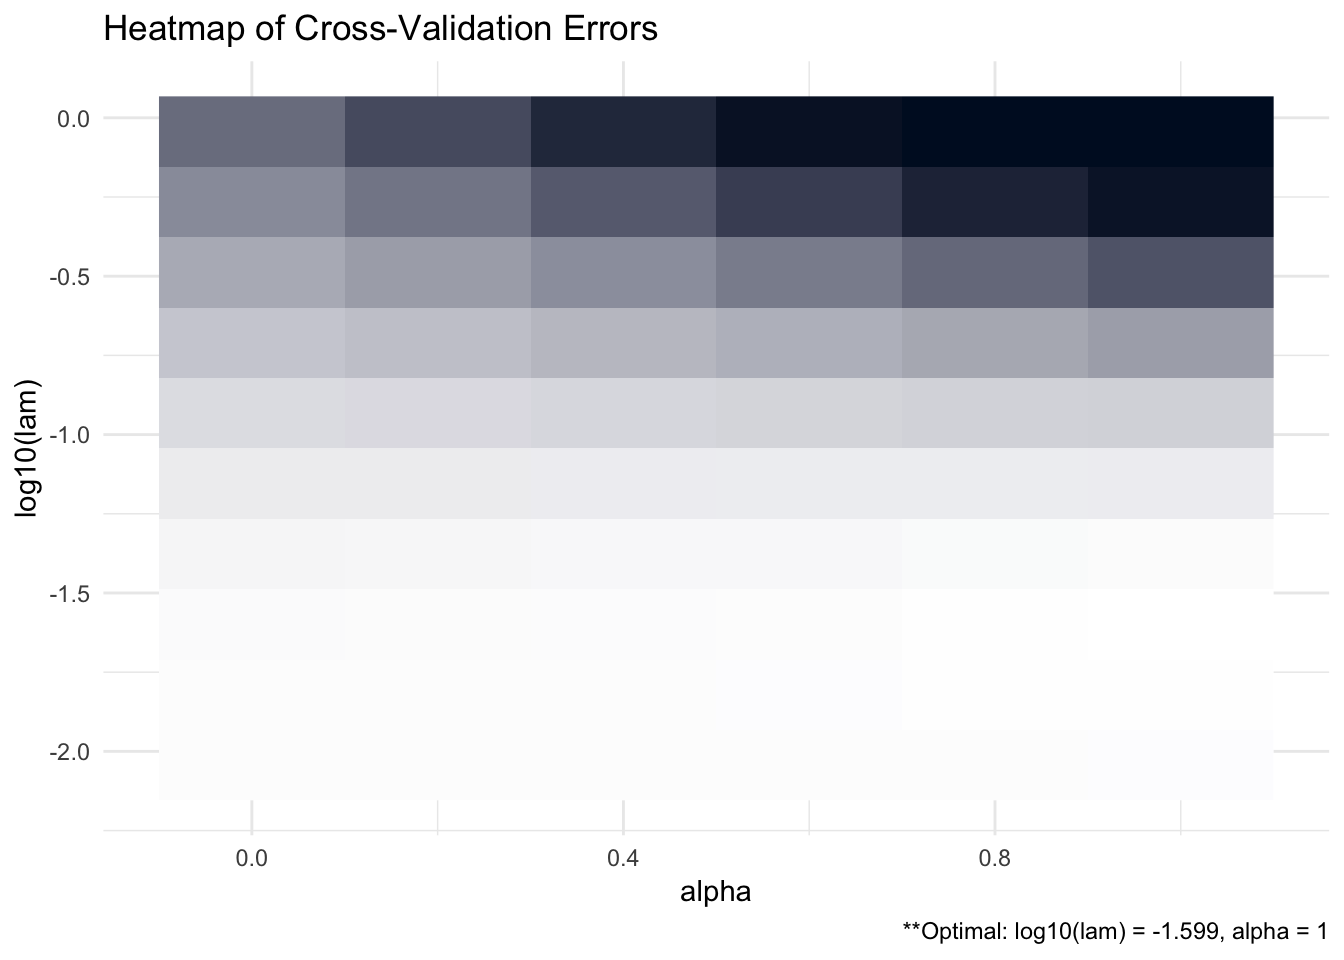
\includegraphics[width=0.8\linewidth,]{Manuscript_files/figure-latex/ADMMsigmapackage1-1} 

}

\caption{CV heatmap for ADMMsigma tutorial.}\label{fig:ADMMsigmapackage1}
\end{figure}

\begin{Shaded}
\begin{Highlighting}[]
\CommentTok{# produce line graph for CV errors for ADMMsigma}
\KeywordTok{plot}\NormalTok{(ADMM, }\DataTypeTok{type =} \StringTok{"line"}\NormalTok{)}
\end{Highlighting}
\end{Shaded}

\begin{figure}

{\centering 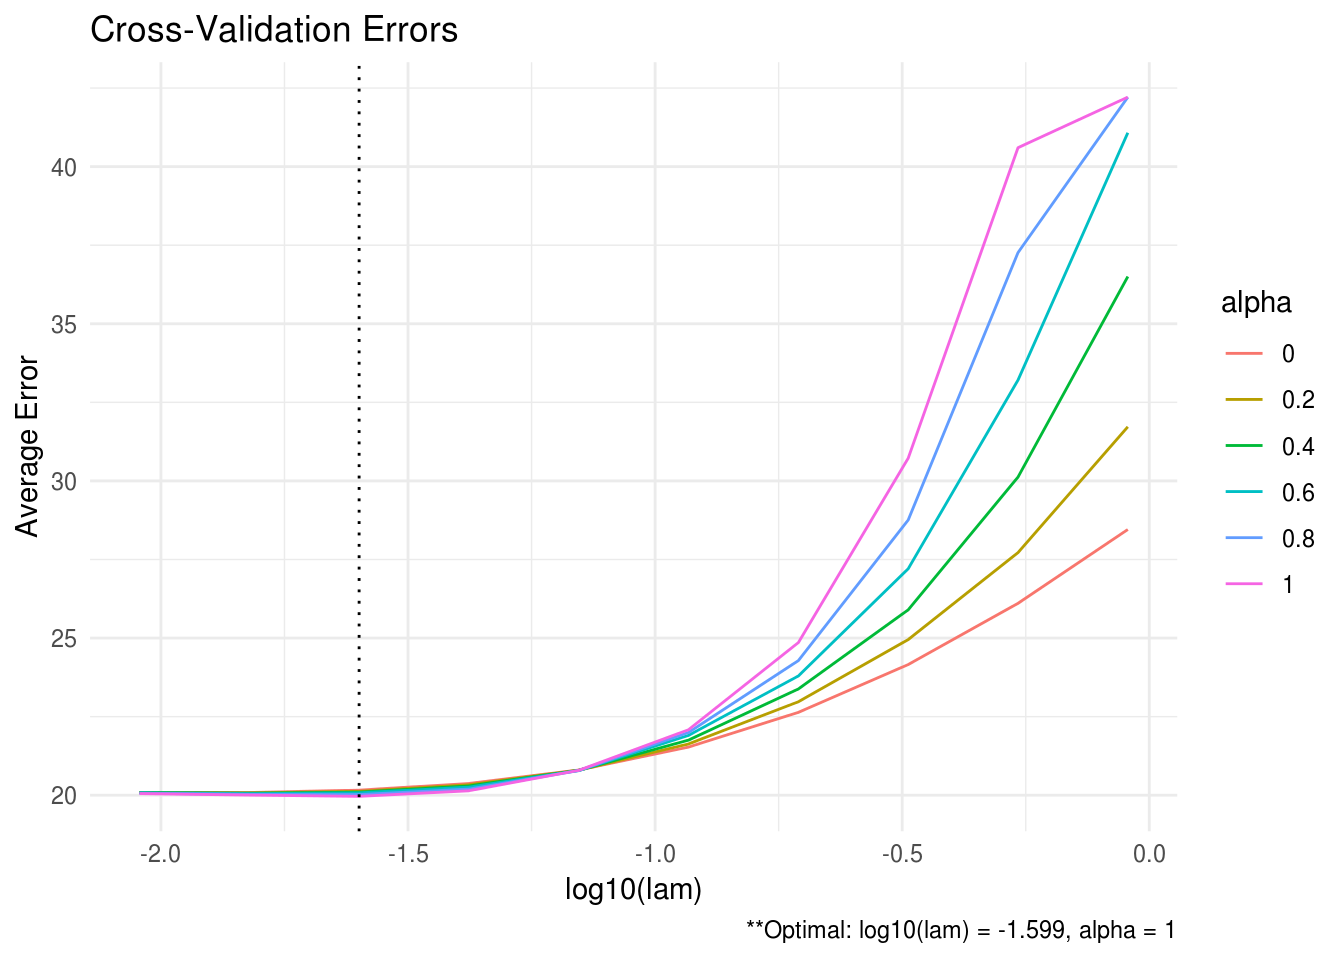
\includegraphics[width=0.8\linewidth,]{Manuscript_files/figure-latex/ADMMsigmapackage2-1} 

}

\caption{CV line graph for ADMMsigma tutorial.}\label{fig:ADMMsigmapackage2}
\end{figure}

\vspace{0.5cm}

\texttt{ADMMsigma} has a number of more advanced options such as cross validation criteria, regularization path, and parallel CV that are explained in more detail on the project website at \href{http://mattxgalloway.com/ADMMsigma/}{mattxgalloway.com/ADMMsigma}.

\hypertarget{scpme-r-package}{%
\chapter{\texorpdfstring{\texttt{SCPME} R Package}{SCPME R Package}}\label{scpme-r-package}}

\texttt{SCPME} is an R package that estimates a penalized precision matrix via a modified alternating direction method of multipliers (ADMM) algorithm as described in \citet{molstad2017shrinking}. Specifically, the modified ADMM algorithm solves the following optimization problem:

\[ \hat{\Omega} = \arg\min_{\Omega \in S_{+}^{p}}\left\{ tr\left(S \Omega\right) - \log\det\left(\Omega\right) + \lambda\left\| A\Omega B - C \right\|_{1} \right\} \]

where \(\lambda > 0\) is a tuning parameter, \(A, B, \mbox{ and } C\) are known, user-specified matrices, and we define \(\left\|A \right\|_{1} = \sum_{i, j} \left| A_{ij} \right|\).

This form of penalty leads to many new, interesting, and novel estimators for the precision matrix \(\Omega\). Users can construct matrices \(A, B, \mbox{ and } C\) so that emphasis is placed on the sum, absolute value of a \emph{characteristic} of \(\Omega\). We will explore a few of these estimators in the tutorial section.

A list of functions contained in the package can be found below:

\begin{itemize}
\item
  \texttt{shrink()} computes the estimated precision matrix
\item
  \texttt{data\_gen()} data generation function (for convenience)
\item
  \texttt{plot.shrink()} produces a heat map or optional line graph for the cross validation errors
\end{itemize}

\hypertarget{installation-1}{%
\section{Installation}\label{installation-1}}

\begin{Shaded}
\begin{Highlighting}[]
\CommentTok{# The easiest way to install is from CRAN}
\KeywordTok{install.packages}\NormalTok{(}\StringTok{"SCPME"}\NormalTok{)}

\CommentTok{# You can also install the development version from GitHub:}
\CommentTok{# install.packages('devtools')}
\NormalTok{devtools}\OperatorTok{::}\KeywordTok{install_github}\NormalTok{(}\StringTok{"MGallow/SCPME"}\NormalTok{)}
\end{Highlighting}
\end{Shaded}

\vspace{0.5cm}

This package is hosted on Github at \href{https://github.com/MGallow/SCPME}{github.com/MGallow/SCPME}. The project website is located at \href{http://mattxgalloway.com/SCPME/}{mattxgalloway.com/SCPME}.

\hypertarget{tutorial-1}{%
\section{Tutorial}\label{tutorial-1}}

The primary function in the \texttt{SCPME} package is \texttt{shrink()}. The input values \(X\) is an \(n \times p\) data matrix so that there are \(n\) rows each representing an observation and \(p\) columns each representing a unique variable and \(Y\) is an \(n \times r\) response matrix where \(r\) is the dimension of the response vector. By default, \texttt{SCPME} will estimate \(\Omega\) using a lasso penalty (\(A = I_{p}, B = I_{p}, \mbox{ and } C = 0\)) and choose the optimal \(\lambda\) tuning parameter that minimizes the mean squared prediction error for the regression of the variable \(Y\) on \(X\) (here \(I_{p}\) denotes a \(p\)-dimension identity matrix). If \(Y\) is not provided, then tuning parameter selection will be based on the validation likelihood. Note that \(\Omega\) (perhaps better denoted here as \(\Omega_{x}\)) will only have meaningful shrinkage unless the data vector \(X \in \mathbb{R^{p}}\) is multi-dimensional (\(p > 1\)).

In this example, the data matrix is \(100 \times 5\) and the response is generated according to the following model:

\[ Y_{i} = \beta'X_{i} + E_{i} \]

where \(E_{i} \sim N\left( 0, 1 \right)\) and \(X_{i}\) is generated from a multivariate normal distribution with mean zero and tapered oracle covariance matrix \(S\). A tapered covariance matrix has the property that its inverse - the precision matrix - is tri-diagonal. Estimating this oracle precision matrix well and efficiently will be our primary interest. In addition, \(\beta\) is randomly generated and sparse. The data will be generated using the \texttt{data\_gen()} function contained in the package.

\vspace{0.5cm}

\begin{Shaded}
\begin{Highlighting}[]
\KeywordTok{library}\NormalTok{(SCPME)}
\KeywordTok{set.seed}\NormalTok{(}\DecValTok{123}\NormalTok{)}

\CommentTok{# generate 100 x 5 X data matrix and 100 x 1 Y data matrix}
\NormalTok{data =}\StringTok{ }\KeywordTok{data_gen}\NormalTok{(}\DataTypeTok{p =} \DecValTok{5}\NormalTok{, }\DataTypeTok{n =} \DecValTok{100}\NormalTok{, }\DataTypeTok{r =} \DecValTok{1}\NormalTok{)}

\CommentTok{# the oracle regression coefficients are sparse}
\NormalTok{data}\OperatorTok{$}\NormalTok{betas}
\end{Highlighting}
\end{Shaded}

\begin{verbatim}
##             [,1]
## [1,] -0.25065233
## [2,]  0.00000000
## [3,]  0.69707555
## [4,]  0.03153231
## [5,]  0.00000000
\end{verbatim}

\vspace{0.5cm}

\begin{Shaded}
\begin{Highlighting}[]
\CommentTok{# shrink sum absolute entries in omega}
\KeywordTok{shrink}\NormalTok{(}\DataTypeTok{X =}\NormalTok{ data}\OperatorTok{$}\NormalTok{X, }\DataTypeTok{Y =}\NormalTok{ data}\OperatorTok{$}\NormalTok{Y)}
\end{Highlighting}
\end{Shaded}

\begin{verbatim}
## 
## Call: shrink(X = data$X, Y = data$Y)
## 
## Iterations: 37
## 
## Tuning parameters:
##       log10(lam)    lam
## [1,]      -1.163  0.069
## 
## Log-likelihood: -178.20154
## 
## Omega:
##          [,1]     [,2]     [,3]     [,4]     [,5]
## [1,]  1.60847 -0.73553 -0.14094 -0.04329 -0.11730
## [2,] -0.73553  1.66045 -0.52579 -0.03576 -0.03342
## [3,] -0.14094 -0.52579  1.73410 -0.85121 -0.07332
## [4,] -0.04329 -0.03576 -0.85121  2.02541 -0.93612
## [5,] -0.11730 -0.03342 -0.07332 -0.93612  1.62397
\end{verbatim}

\vspace{0.5cm}

Notice here that the estimated precision matrix is \emph{not} sparse. This is due to the fact that our cross validation criteria is the mean-squared prediction error. We can estimate a new precision matrix using the validation likelihood as the cross validation criteria with the following command:

\vspace{0.5cm}

\begin{Shaded}
\begin{Highlighting}[]
\CommentTok{# shrink sum absolute entries in omega}
\KeywordTok{shrink}\NormalTok{(}\DataTypeTok{X =}\NormalTok{ data}\OperatorTok{$}\NormalTok{X, }\DataTypeTok{Y =}\NormalTok{ data}\OperatorTok{$}\NormalTok{Y, }\DataTypeTok{crit.cv =} \StringTok{"loglik"}\NormalTok{)}
\end{Highlighting}
\end{Shaded}

\begin{verbatim}
## 
## Call: shrink(X = data$X, Y = data$Y, crit.cv = "loglik")
## 
## Iterations: 51
## 
## Tuning parameters:
##       log10(lam)    lam
## [1,]      -2.163  0.007
## 
## Log-likelihood: -120.02858
## 
## Omega:
##          [,1]     [,2]     [,3]     [,4]     [,5]
## [1,]  2.11926 -1.17294 -0.13784 -0.00678 -0.20014
## [2,] -1.17294  2.28420 -0.81629  0.00009 -0.00001
## [3,] -0.13784 -0.81629  2.45520 -1.42117  0.01650
## [4,] -0.00678  0.00009 -1.42117  3.09526 -1.56839
## [5,] -0.20014 -0.00001  0.01650 -1.56839  2.24703
\end{verbatim}

\vspace{0.5cm}

All of the estimators so far have used a lasso penalty that penalizes the sum of the absolute value of all the entries in \(\Omega\) (\(A = I_{p}, B = I_{p}, \mbox{ and } C = 0\)). In effect, this penalty embeds an assumption in our estimate that the true population precision matrix, \(\Omega\), is sparse. The flexibility of the penalty described in \citet{molstad2017shrinking} allows us to make other assumptions as well. For instance, in the penalty we could set \(A = I_{p}, B = \Sigma_{xy}\) where \(\Sigma_{xy}\) is the covariance matrix of \(X\) and \(Y\), and \(C = 0\). In which case our penalty function

\[P_{\lambda}\left(\Omega \right) = \lambda\left\| A\Omega B - C \right\|_{1} = \lambda\left\| \Omega\Sigma_{xy} \right\|_{1} = \lambda\left\| \beta \right\|_{1} \]

This objective function estimates an \(\Omega\) via the marginal log-likelihood of \(X\) under the assumption that the forward regression coefficient \(\beta\) is sparse (recall that \(\beta \equiv \Omega\Sigma_{xy}\)). Of course, in practice, we do not know the true covariance matrix \(\Sigma_{xy}\) but we might consider using the sample estimate \(\hat{\Sigma}_{xy} = \sum_{i = 1}^{n}\left(X_{i} - \bar{X}\right)\left(Y_{i} - \bar{Y}\right)'/n\).

\vspace{0.5cm}

\begin{Shaded}
\begin{Highlighting}[]
\CommentTok{# assume sparsity in beta}
\NormalTok{lam_max =}\StringTok{ }\KeywordTok{max}\NormalTok{(}\KeywordTok{abs}\NormalTok{(}\KeywordTok{crossprod}\NormalTok{(data}\OperatorTok{$}\NormalTok{X, data}\OperatorTok{$}\NormalTok{Y)))}
\NormalTok{(}\DataTypeTok{shrink =} \KeywordTok{shrink}\NormalTok{(}\DataTypeTok{X =}\NormalTok{ data}\OperatorTok{$}\NormalTok{X, }\DataTypeTok{Y =}\NormalTok{ data}\OperatorTok{$}\NormalTok{Y, }\DataTypeTok{B =} \KeywordTok{cov}\NormalTok{(data}\OperatorTok{$}\NormalTok{X, data}\OperatorTok{$}\NormalTok{Y), }
    \DataTypeTok{lam.max =}\NormalTok{ lam_max, }\DataTypeTok{nlam =} \DecValTok{20}\NormalTok{))}
\end{Highlighting}
\end{Shaded}

\begin{verbatim}
## 
## Call: shrink(X = data$X, Y = data$Y, B = cov(data$X, data$Y), nlam = 20, 
##     lam.max = lam_max)
## 
## Iterations: 84
## 
## Tuning parameters:
##       log10(lam)    lam
## [1,]      -0.167  0.681
## 
## Log-likelihood: -133.98097
## 
## Omega:
##          [,1]     [,2]     [,3]     [,4]     [,5]
## [1,]  2.12467 -1.20016 -0.01149  0.01660 -0.20424
## [2,] -1.20016  2.28202 -0.70370  0.03047 -0.01211
## [3,] -0.01149 -0.70370  2.09284 -1.47505  0.01020
## [4,]  0.01660  0.03047 -1.47505  2.86829 -1.45784
## [5,] -0.20424 -0.01211  0.01020 -1.45784  2.18752
\end{verbatim}

Note that we specified the maximum \texttt{lam} value in the previous function to expand the tuning parameter grid. With these settings, the augmented ADMM algorithm also solves for the estimated \(\beta\) coefficient matrix simultaneously:

\vspace{0.5cm}

\begin{Shaded}
\begin{Highlighting}[]
\CommentTok{# print estimated beta matrix}
\NormalTok{shrink}\OperatorTok{$}\NormalTok{Z}
\end{Highlighting}
\end{Shaded}

\begin{verbatim}
##            [,1]
## [1,] 0.00000000
## [2,] 0.00000000
## [3,] 0.42221120
## [4,] 0.04782093
## [5,] 0.00000000
\end{verbatim}

\vspace{0.5cm}

Another possible penalty is to set \(B = \left[ \Sigma_{xy}, I_{p} \right]\) so that the identity matrix is appended to the covariance matrix of \(X\) and \(Y\). That is, the penalty \(P\), is constructed as

\[ P_{\lambda}\left(\Omega \right) = \lambda\left\| A\Omega B - C \right\|_{1} = \lambda\left\| \Omega\left[\Sigma_{xy}, I_{p}\right] \right\|_{1} = \lambda\left\| \beta \right\|_{1} + \lambda\left\| \Omega \right\|_{1} \]

In this case, we are equally penalizing the sum, absolute values of entries in \(\beta\) \emph{and} \(\Omega\) which embeds an assumption that \(\beta\) and \(\Omega\) are both sparse.

\vspace{0.5cm}

\begin{Shaded}
\begin{Highlighting}[]
\CommentTok{# assume sparsity in beta AND omega}
\NormalTok{(}\DataTypeTok{shrink =} \KeywordTok{shrink}\NormalTok{(}\DataTypeTok{X =}\NormalTok{ data}\OperatorTok{$}\NormalTok{X, }\DataTypeTok{Y =}\NormalTok{ data}\OperatorTok{$}\NormalTok{Y, }\DataTypeTok{B =} \KeywordTok{cbind}\NormalTok{(}\KeywordTok{cov}\NormalTok{(data}\OperatorTok{$}\NormalTok{X, }
\NormalTok{    data}\OperatorTok{$}\NormalTok{Y), }\KeywordTok{diag}\NormalTok{(}\KeywordTok{ncol}\NormalTok{(data}\OperatorTok{$}\NormalTok{X))), }\DataTypeTok{lam.max =} \DecValTok{10}\NormalTok{, }\DataTypeTok{lam.min.ratio =} \FloatTok{1e-04}\NormalTok{, }
    \DataTypeTok{nlam =} \DecValTok{20}\NormalTok{))}
\end{Highlighting}
\end{Shaded}

\begin{verbatim}
## 
## Call: shrink(X = data$X, Y = data$Y, B = cbind(cov(data$X, data$Y), 
##     diag(ncol(data$X))), nlam = 20, lam.max = 10, lam.min.ratio = 1e-04)
## 
## Iterations: 46
## 
## Tuning parameters:
##       log10(lam)    lam
## [1,]       0.368  2.336
## 
## Log-likelihood: -624.54758
## 
## Omega:
##          [,1]     [,2]     [,3]     [,4]     [,5]
## [1,]  0.26376 -0.00003 -0.00015 -0.00010 -0.00005
## [2,] -0.00003  0.24002 -0.00017 -0.00012 -0.00006
## [3,] -0.00015 -0.00017  0.19066 -0.00516 -0.00020
## [4,] -0.00010 -0.00012 -0.00516  0.20362 -0.00014
## [5,] -0.00005 -0.00006 -0.00020 -0.00014  0.22750
\end{verbatim}

\begin{Shaded}
\begin{Highlighting}[]
\CommentTok{# print estimated beta}
\NormalTok{shrink}\OperatorTok{$}\NormalTok{Z[, }\DecValTok{1}\NormalTok{, drop =}\StringTok{ }\OtherTok{FALSE}\NormalTok{]}
\end{Highlighting}
\end{Shaded}

\begin{verbatim}
##            [,1]
## [1,] 0.06389361
## [2,] 0.08542992
## [3,] 0.14200713
## [4,] 0.12357129
## [5,] 0.09958374
\end{verbatim}

\vspace{0.5cm}

\texttt{SCPME} also has the capability to provide plots (heatmaps and line graphs) for the cross validation errors. In the heatmap plot below, the more bright, white areas correspond to a better tuning parameter selection (lower cross validation error).

\vspace{0.5cm}

\begin{Shaded}
\begin{Highlighting}[]
\CommentTok{# produce CV heat map}
\KeywordTok{plot}\NormalTok{(shrink, }\DataTypeTok{type =} \StringTok{"heatmap"}\NormalTok{)}
\end{Highlighting}
\end{Shaded}

\begin{figure}

{\centering 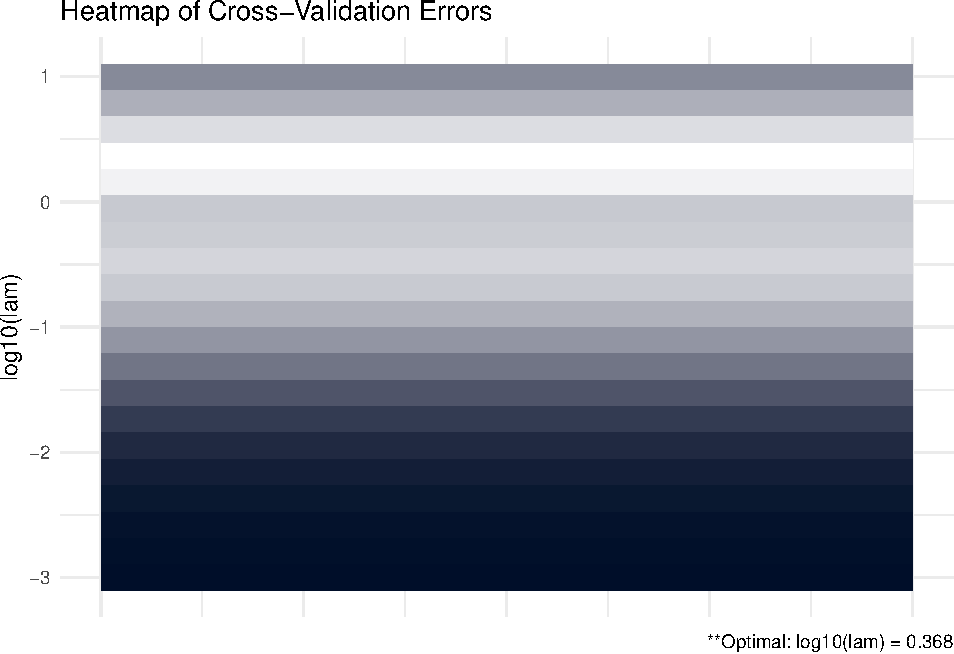
\includegraphics[width=0.8\linewidth,]{Manuscript_files/figure-latex/SCPMEpackage1-1} 

}

\caption{CV heatmap for SCPME tutorial}\label{fig:SCPMEpackage1}
\end{figure}

\begin{Shaded}
\begin{Highlighting}[]
\CommentTok{# produce line graph}
\KeywordTok{plot}\NormalTok{(shrink, }\DataTypeTok{type =} \StringTok{"line"}\NormalTok{)}
\end{Highlighting}
\end{Shaded}

\begin{figure}

{\centering 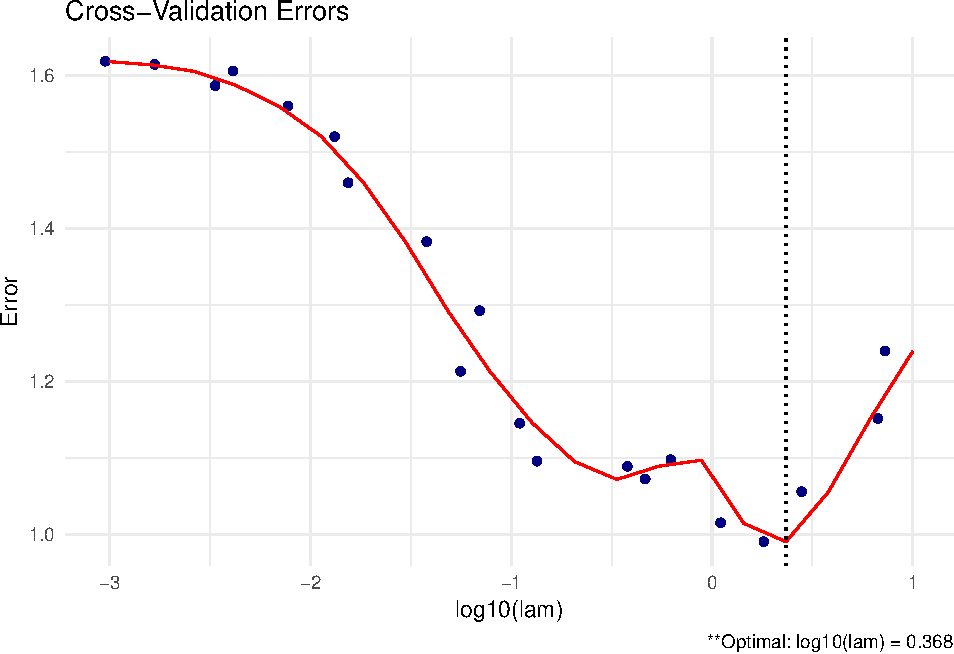
\includegraphics[width=0.8\linewidth,]{Manuscript_files/figure-latex/SCPMEpackage2-1} 

}

\caption{CV line graph for SCPME tutorial}\label{fig:SCPMEpackage2}
\end{figure}

\vspace{0.5cm}

\texttt{SCPME} has a number of more advanced options including alternative convergence criteria and parallel CV that are explained in detail on the project website at \href{http://mattxgalloway.com/SCPME/}{mattxgalloway.com/SCPME}.

\bibliography{lib.bib,packages.bib}

\end{document}
